%%
%% This is file `sample-sigconf.tex',
%% generated with the docstrip utility.
%%
%% The original source files were:
%%
%% samples.dtx  (with options: `sigconf')
%% 
%% IMPORTANT NOTICE:
%% 
%% For the copyright see the source file.
%% 
%% Any modified versions of this file must be renamed
%% with new filenames distinct from sample-sigconf.tex.
%% 
%% For distribution of the original source see the terms
%% for copying and modification in the file samples.dtx.
%% 
%% This generated file may be distributed as long as the
%% original source files, as listed above, are part of the
%% same distribution. (The sources need not necessarily be
%% in the same archive or directory.)
%%
%% The first command in your LaTeX source must be the \documentclass command.
\documentclass[sigconf]{acmart}
%% NOTE that a single column version may be required for 
%% submission and peer review. This can be done by changing
%% the \doucmentclass[...]{acmart} in this template to 
%% \documentclass[manuscript,screen]{acmart}
%% 
%% To ensure 100% compatibility, please check the white list of
%% approved LaTeX packages to be used with the Master Article Template at
%% https://www.acm.org/publications/taps/whitelist-of-latex-packages 
%% before creating your document. The white list page provides 
%% information on how to submit additional LaTeX packages for 
%% review and adoption.
%% Fonts used in the template cannot be substituted; margin 
%% adjustments are not allowed.
%%
%%
%% \BibTeX command to typeset BibTeX logo in the docs
\usepackage{graphicx, caption, subcaption}
\usepackage{amsmath}
\usepackage{color}
\usepackage{multirow}
\usepackage{booktabs}
\usepackage{bbm}
\usepackage{enumitem}
\usepackage[flushleft]{threeparttable}
\usepackage{makecell}
\usepackage{ulem}

\AtBeginDocument{%
  \providecommand\BibTeX{{%
    \normalfont B\kern-0.5em{\scshape i\kern-0.25em b}\kern-0.8em\TeX}}}

%% Rights management information.  This information is sent to you
%% when you complete the rights form.  These commands have SAMPLE
%% values in them; it is your responsibility as an author to replace
%% the commands and values with those provided to you when you
%% complete the rights form.
\setcopyright{acmcopyright}
\copyrightyear{2021}
\acmYear{2021}
\acmDOI{10.1145/1122445.1122456}

%% These commands are for a PROCEEDINGS abstract or paper.
\acmConference[SIGIR '21]{ACM SIGIR Conference on Research and Development in Information Retrieval}{July 11--15, 2021}{Virtual Event}
\acmBooktitle{ACM SIGIR Conference on Research and Development in Information Retrieval, July 11--15, 2021, Virtual Event}
\acmPrice{15.00}
\acmISBN{978-1-4503-XXXX-X/18/06}


%%
%% Submission ID.
%% Use this when submitting an article to a sponsored event. You'll
%% receive a unique submission ID from the organizers
%% of the event, and this ID should be used as the parameter to this command.
\acmSubmissionID{168}
\newcommand{\secref}[1]{Section \ref{#1}}
\newcommand{\figref}[1]{Figure \ref{#1}}
\newcommand{\eqnref}[1]{Eq. (\ref{#1})}
\newcommand{\tabref}[1]{Table \ref{#1}}
\newcommand{\exref}[1]{Example \ref{#1}}
\newcommand{\cut}[1]{}
\DeclareMathOperator*{\argmax}{argmax} % thin space, limits underneath in displays
\DeclareMathOperator*{\argmin}{argmin}

\newcommand{\KZ}[1]{\textcolor{blue}{Kenny: #1}}

% \renewcommand{\cmidrulesep}{0mm} 
% \setlength{\aboverulesep}{0mm} 
% \setlength{\belowrulesep}{0mm} 
% \setlength{\abovetopsep}{0cm} 
% \setlength{\belowbottomsep}{0cm}
\newcommand{\tabincell}[2]{\begin{tabular}{@{}#1@{}}#2\end{tabular}}

%%
%% The majority of ACM publications use numbered citations and
%% references.  The command \citestyle{authoryear} switches to the
%% "author year" style.
%%
%% If you are preparing content for an event
%% sponsored by ACM SIGGRAPH, you must use the "author year" style of
%% citations and references.
%% Uncommenting
%% the next command will enable that style.
%%\citestyle{acmauthoryear}

%%
%% end of the preamble, start of the body of the document source.
\begin{document}

%%
%% The "title" command has an optional parameter,
%% allowing the author to define a "short title" to be used in page headers.
\title{Modeling Implicit User Feedback in Anonymous Session-based 
News Recommendation}

%%
%% The "author" command and its associated commands are used to define
%% the authors and their affiliations.
%% Of note is the shared affiliation of the first two authors, and the
%% "authornote" and "authornotemark" commands
%% used to denote shared contribution to the research.
% \author{Gong Shansan}
% \affiliation{%
%  \institution{Shanghai Jiao Tong University}
%  \streetaddress{800 Dongchuan Rd}
%  \city{Shanghai}
%  \postcode{200240}
%  \country{China}}
% \email{gongshansan@sjtu.edu.cn}

% \author{Julius P. Kumquat}
% \affiliation{%
%   \institution{The Kumquat Consortium}
%   \city{New York}
%   \country{USA}}
% \email{jpkumquat@consortium.net}

%%
%% By default, the full list of authors will be used in the page
%% headers. Often, this list is too long, and will overlap
%% other information printed in the page headers. This command allows
%% the author to define a more concise list
%% of authors' names for this purpose.
% \renewcommand{\shortauthors}{Gong Shansan, et al.}

%%
%% The abstract is a short summary of the work to be presented in the
%% article.
\begin{abstract}
% News articles are generated every day in online news platforms, and meanwhile many users are using their temporary account without login or within a short session. This set challenges for the existing news recommendation system to extract short term intentions of the user with limited and implicit feedback information. 
News recommendation for anonymous users is useful on
many news portals. It is challenging because both the life
span of news articles and the duration of user visits are short.
This work proposes a method to model user behavior and preferences from their implicit feedback, using content and temporal information of the articles and user clicks.
Empirical evaluation on three real-world news datasets shows 
that the method not only mitigates the cold-start problem and 
improves the diversity of recommendation, but also 
makes more accurate predictions than all recent state-of-the-art 
session-based recommendation approaches.

%Many online news platforms allow anonymous user login, and this set challenges for the existing news recommendation system to extract immediate interests of the user with limited implicit feedback information. This session-based recommendation  usually be modeled as next-item prediction task in recent work, but most of them regard click as positive feedback, ignoring other informative user behaviours.
%  When a user clicks an article, does this mean he really likes it? Does this mean he really doesn't like the others articles? These two questions encourage us to exploit user's refined positive/negative implicit feedback and to dig out user's deep intentions.
%  
% Some promising results have been recently achieved by formulating recommendation problem sequentially, and the usage of Deep Learning techniques such as RNN and multi-head attention transformer highlights their effectiveness in extracting sequential information. However, in news recommendation domain, article-cold-start problem and recommendation diversity need to be taken into account. In this paper we design time and context-aware session-based news recommendation methods that consider real scenes to produce the rich and user-interested recommendation list. 
  % As the positive implicit feedback, the interval that user stays for each article represents user's different preference, while the articles that user doesn't click in user's impression list pass more strong negative information than other articles. 
%We design a novel Implicit feedback based Time \& Content Aware Recommendation system (ITCAR), which leverages on the implicit feedback from user combined with temporal \& content information, trying to capture the hidden feature of within-session browsing behaviour. 

  % The temporal information contains click-level and session-levelinformation, trying to capture the feature of within-session brows-ing behaviour. The context of user interactions including article con-tent and session impression, is introduced to collect topic-orientedinterests.
  

\end{abstract}

%%
%% The code below is generated by the tool at http://dl.acm.org/ccs.cfm.
%% Please copy and paste the code instead of the example below.
%%
\begin{CCSXML}
  <ccs2012>
     <concept>
         <concept_id>10002951.10003317.10003347.10003350</concept_id>
         <concept_desc>Information systems~Recommender systems</concept_desc>
         <concept_significance>500</concept_significance>
         </concept>
%     <concept>
%         <concept_id>10010147.10010257.10010293.10010294</concept_id>
%         <concept_desc>Computing methodologies~Neural networks</concept_desc>
%         <concept_significance>500</concept_significance>
%         </concept>
   </ccs2012>
\end{CCSXML}

\ccsdesc[500]{Information systems~Recommender systems}
%\ccsdesc[500]{Computing methodologies~Neural networks}

%%
%% Keywords. The author(s) should pick words that accurately describe
%% the work being presented. Separate the keywords with commas.
\keywords{news recommendation, session-based, implicit feedback,
time aware, cold-start}

%%
%% This command processes the author and affiliation and title
%% information and builds the first part of the formatted document.
\maketitle
\section{Introduction}
\label{sec:intro}

Evaluation of dialogue systems is an open problem. Existing
automatic evaluation metrics for chitchat systems are similar to those for 
other text generation tasks (e.g., machine translation \citep{papineni-etal-2002-bleu}, question-answering \citep{rajpurkar-etal-2016-squad}, 
summarization \citep{lin-2004-rouge}), which depends on calculating word 
overlaps with reference responses. 
However, for chitchats, there are usually 
many alternative but plausible responses given a situation, 
perhaps more than any other text generation task mentioned above. 
A limited number of reference responses are 
not sufficient to determine how good a generated response is. 
Moreover, such static settings are not good at
assessing an interactive, context-sensitive system.

Interactive human evaluation metrics usually 
involve a Likert scale evaluation after a multi-turn conversation 
with the bot to be assessed. 
While this method is a step up from the previous static evaluation, 
it is difficult for human judges to give a concrete score to
any bot.
%\KZ{But are we also asking judges to score invidividual bots, which is difficult?} 
Comparing the performance of two bots is easier. 
Thus ACUTE-EVAL~\citep{DBLP:journals/corr/abs-1909-03087} asks the 
judges to make a binary judgment of who is better in conversations between two identical bots 
or between a human and a bot. A more advanced version of that
is \textit{Spot The Bot}~\cite{deriu-etal-2020-spot} which models the 
human evaluation of a 
conversation after the Turing test. However, such a process is still 
time-consuming and costly, compared with automatic evaluations.

In our opinion, a good method for evaluating multi-turn 
conversational model/system 
should satisfy the following requirements:
i) be as efficient and inexpensive as possible;
ii) can truly reflect a model's ability to conduct a human conversation; 
iii) evaluation results should correlate well with human judgments;
iv) can be used to compare and rank the capabilities of a set of models/systems.
  
Toward that goal, in this work, we propose an automatic interactive evaluation 
framework, which is called \textit{ChatMatch}(CM) for chitchat
agents. This framework can be used to rank a number of bots with little
time and minimum human effort.  Above all, we want to emphasize 
the significance of direct interactions between bots 
in the evaluation.
%\textcolor{red}{Reviewer 1 said that he didn't understand this sentence. Maybe remove "the observation"?} 
People tend to believe that human-bot conversations are more reliable 
and produce more comprehensive evaluations of chatbots' capabilities. 
This is not always true. As human annotators know their counterpart is a robot, 
they tend to ask common and goal-directed questions. 
On the other hand, some bot-bot chat logs in our experiments show that, 
surprisingly, conversations between different bots may expose their strengths 
and weaknesses never seen in human-bot conversations. 
\figref{fig:two convs} gives two small chat fragments, illustrating such
differences.
While talking about hobbies, human keeps asking the bot some blunt
questions, which leads to dull responses from the bot.
However, in a bot-bot setting, two bots, including the same bot in the previous
conversation, start explaining their hobbies to each other, producing a more
interesting conversation. 

\begin{figure}[ht!]
 \centering

% \subfigure[Chat snippet between human and bot (Plato-2)]{
\subfigure[Chat snippet between human and bot]{ 
 %  \centering
  %  \begin{minipage}[t]{0.5\linewidth}
  \includegraphics[width=0.95\linewidth]{eg4.eps}\label{fig:sub-first}
  %  \end{minipage}
 }
 
 \subfigure[Chat snippet between two bots]{
  % \centering
  % \begin{minipage}[t]{0.5\linewidth}
  \includegraphics[width=0.95\linewidth]{figs.eps}\label{fig:sub-second}
  % \end{minipage}
 }
 \caption{Snippets from human-bot and bot-bot chat logs}
\label{fig:two convs}
\end{figure}

Our framework consists of two components: \textit{competition} and 
\textit{scoring}, which interoperate with each other. 
The competition is modeled
after most sports tournaments such as soccer or ping pong. 
There are three levels of competitions. From bottom up, they are:
game-level, match-level and tournament-level. 
Each match consists of several games. During a game, two bots will converse 
freely with each other and a virtual judge will score their performances 
according to a set of user-defined criteria such as consistency and fluency, 
etc.  These criteria are flexible and extensible.
%As an example like \figref{fig:example} shows, 
%Bot $A$ will be 
%penalized twice for repeating while Bot $B$ will be penalized once for 
%contradicting itself. In addition to the penalty, 
%a bonus point is rewarded to $A$
%who shows to produce relevant response with long term memory. 
%\KZ{Do we still have this as a criterion?}
%However, the specific bonus and penalty settings may vary 
%depending on the domain and scenarios that the experiment is 
%set in. 

%\begin{figure}[th!]
%	\centering
%	\includegraphics[width=0.95\columnwidth]{example.eps}
%	\caption{A chat snippet between two bots.}
%	\label{fig:example}
%\end{figure}

The main contributions of this paper are:
\begin{itemize}
\item We propose the first interactive evaluation framework for chatbots which
is based solely on bot-bot conversations and modeled after sports competitions (\secref{sec:competition}).
\item We designed three algorithms to score \textit{diversity}, \textit{consistency}, \textit{relevance}, three important dimensions in a bot's chatting 
abilities.
\item  The entire scoring process is fully automated and efficient. 
In our experiments, the system can rank seven bots in less than 
three minutes on average (\secref{sec:scoring}, \secref{sec:time}).
\item  Our experiments show that the results produced by our framework
closely correlate with the human evaluation results. 
Results also show that our framework outperforms 
several recent strong baseline evaluation systems (\secref{sec:main}).
%\item %We demonstrate the improvements in efficiency 
%using direct chat logs between bots.
%\KZ{Maybe this should not be a contribution but part of the conclusion?}
%We show that the chats between bots are impressively informative, 
%even richer than the chats between humans and bots.
%This suggests some possible directions to improve 
%the capabilities of bots in the future.
%(e.g., by having them learn from each other)  (\secref{sec:diversity})
\end{itemize}

\section{Problem Formulation}
\label{sec:task}

In this section, we formally define the abstractive dialogue summarization
task with mathematical notations. We highlight the characteristics of this task by contrasting it with the well-studied document summarization
problem. Finally, we present a hierarchical classification of application scenarios, demonstrating the practicality of this task.

\subsection{Task Definition}\label{sec:taskdefinition}
A dialogue can be formalized as a sequence of $T$ chronologically ordered turns:
\begin{equation}
	D = \{U_1, U_2, ..., U_T\}
	\label{eq:dialogue}
\end{equation}
Each turn $U_t$ generally consists of a speaker/role $s_t$ and corresponding utterance $u_t = \{w_i^t|_{i=1}^{l_t}\}$. $w_i^t$ represents the $i$-th token\footnote{To construct input for neural models, tokenizers are used to tokenize utterances into tokens in the vocabulary. Rare words may result in multiple tokens by algorithms such as Byte-Pair-Encoding. We do not strictly distinguish words and tokens in this survey.} in the $t$-th utterance, $l_t$ is the length of $u_t$.

Dialogue summarization aims at generating a short but informative 
summary $Y=\{y_1,y_2,...,y_n\}$ for $D$, where $n$ is 
the number of summary tokens. $Y$ represents the reference summary 
and $\hat{Y}$ represents the generated summary.



\subsection{Comparisons to Document Summarization}\label{sec:divergence}

Dialogue summarization is different from document summarization in various 
aspects, including language style and format, information density, 
discourse structure, and topic boundaries.

\begin{figure}[ht]
	\centering
	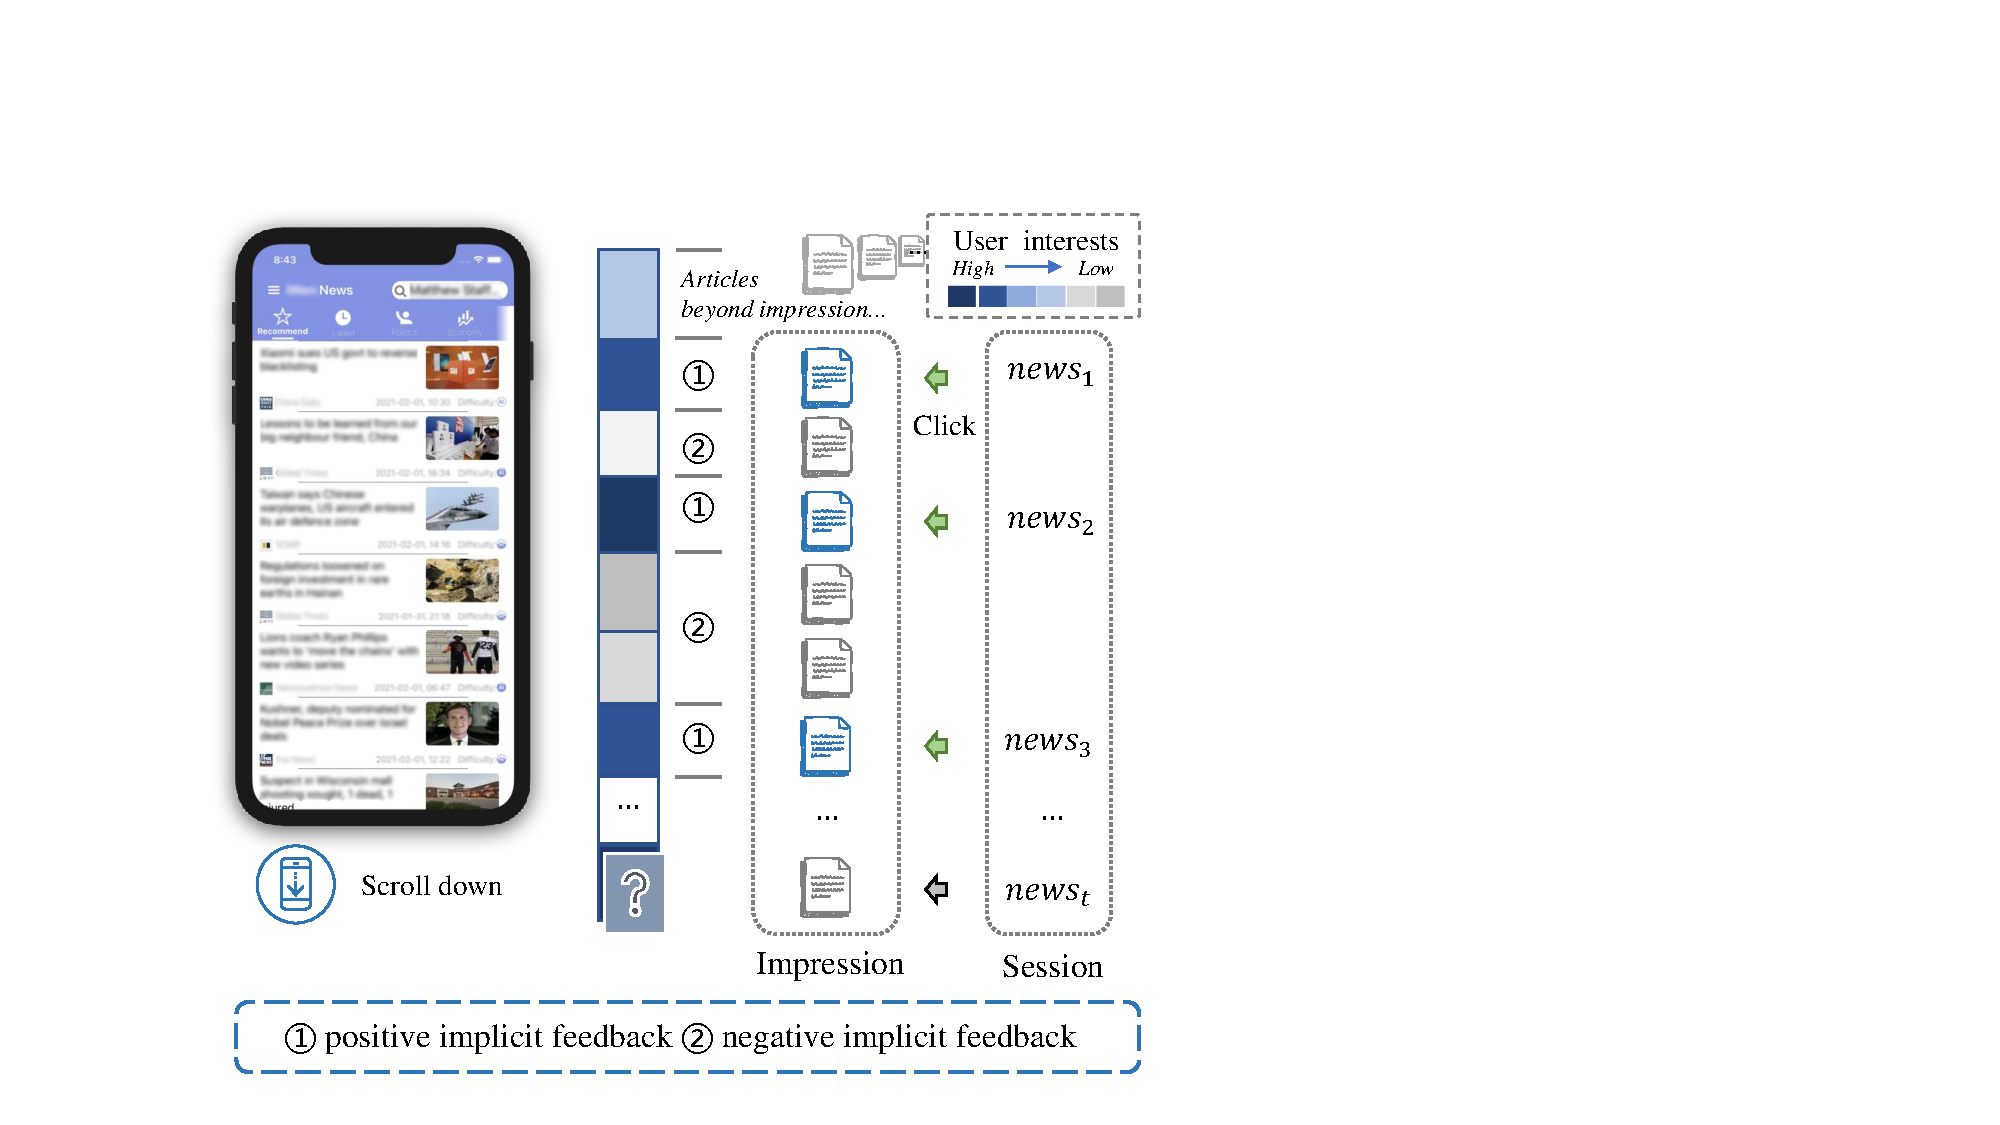
\includegraphics[scale=0.5]{fig/example.pdf}
	\caption{An example multi-party dialogue and its summary. The arrows represent unsequential dependencies between utterances. Elliptical sentences are in italic.}
	\label{fig:example}
\end{figure}

\textbf{Word Level - Language Style and Format:} 
Documents in previous well-researched summarization tasks are written from the third point of view, while dialogues consist of utterances expressed by different speakers in first person. Informal and colloquial expressions are common especially for recorded dialogues from speech, such as ``Whoa'' in $U_6$ and ``u'' representing ``you'' in $U_7$ from Figure~\ref{fig:example}.
Pronouns are frequently used to refer to events or persons mentioned in the dialogue history. Around 72\% of mentions in the conversation are {anaphoras} %pronouns
as stated in \citet{bai2021joint}. Meanwhile, the performance of coreference resolution models trained on normal text drops dramatically on dialogues~\cite{liu2021coreference}. It manifests the existence of language style differences between documents and dialogues, leading to difficulties in understanding the mappings between speakers and events in dialogues.


\textbf{Sentence/Utterance Level - Information Density:}
Document sentences are more self-contained with complete SVO (subject-verb-object) structures, while elliptical utterances are ubiquitous in dialogues, including $U_3$, $U_6$, $U_7$, $U_{11}$ and $U_{12}$.
Besides, the long dialogue can be summarized into a single summary sentence for the example in Figure~\ref{fig:example} as a result of back-and-forth questions and confirmations among speakers for communication purposes.
Question answerings, acknowledgments, and comments~\cite{asher2016discourse} are frequent discourse relations among utterances to narrow down speakers' information gaps and reach agreements.
In this way, dialogue utterances are highly content-dependent, and the information is scattered~\cite{zhang2021exploratory}, raising the difficulties for generating integral contents.

\textbf{Inter-sentence/utterance Level - Discourse structure:}
Articles tend to be well-structured, such as 
general-to-specific structure or deductive order. 
For example, the most important information 
in news summarization are always at the beginning of the document, resulting in a competitive performance of the simple Lead-$3$ baseline~\cite{nallapati2017, see2017get}. However, it is not the same for dialogue summarization. Both Lead-$3$ and Longest-$3$, i.e. $\{U1, U2, U3\}$ and $\{U4, U8, U9\}$ in Figure~\ref{fig:example}, get poor results in different dialogue scenarios~\cite{gliwa2019samsum,chen2021dialsumm,zhang2021emailsum}.
The dependencies among utterances are interleaved, shown by arrows in Figure~\ref{fig:example}, and discourse relations in dialogues are more flexible,
even with the correction of wrong information~\cite{asher2016discourse}. 
For example, 
Jake refused to be available for the reunion in $U_6$, but later agreed
in $U_8$.  As a result, it is more challenging to reason cross utterances for 
dialogue summarization than document summarization.

\textbf{Passage/Session Level - Topic boundaries:} Sentences under the same topic in documents are collected together in a paragraph or a section.
Previous works for extractive~\cite{xiao2019extractive} and abstractive summarization~\cite{cohan2018discourse} both took advantage of such features and made great progress. 
However, a dialogue is a stream of continuous 
utterances without boundaries, even for hours of discussion. The same topic may be discussed repeatedly 
with redundancies and new information, setting up obstacles for content 
selection in dialogue summarization.

%\JQ{it will be good to see the advantages of abstractive vs extractive approaches for dialogue summarization.}
%\JQ{add a little more about extractive methods, and explain why abstractive is more preferred especially in the case of dialogues.}
To better explain why abstractive approaches are more preferred than extractive ones for dialogues, we list the result of the best rule-based extractive baseline, i.e., Longest-$3$~\cite{gliwa2019samsum}, the oracle extractive result determined by Rouge-L Recall score between each summary sentence and dialogue utterances~\cite{chen2018fast}, and the generation by BART fine-tuned on SAMSum dataset~\cite{gliwa2019samsum} of the simple dialogue in Figure~\ref{fig:example} as follows:
\\
\begin{tabular}{|p{1.5cm}|p{\linewidth-2.3cm}|}
	\hline
	\textbf{Longest-$3$} & Jessica: If I move some things around, I can too! Jake: Hell yeah man! You know I freelance, worst case scenario I'll work from wherever we are Jessica: We should meet up where we did last time, it's perfect middle for everyone.\\
	\hline
	\textbf{Oracle} & Jake: Hell yeah man! You know I freelance, worst case scenario I'll work from wherever we are\\
	\hline
	\textbf{BART}& Ted, Pia, Jessica and Jake are going to meet up on Friday night. \\
	\hline
\end{tabular}
\\
We can see that the readability of generated summaries are poor for Longest-$3$ and Oracle due to the language style and format difference. The compression ratio of Longest-$3$ is apparently low while it still misses the involvement of Ted and Pia as a result of low information density of dialogues. Oracle is concise but much more information is missing. Meanwhile, the fine-tuned BART as an abstractive approach shows the favorable performance. Therefore, abstractive approaches becomes the mainstream in researches on dialogue summarization. In a word, dialogue summarization is an valuable research direction in summarization, where the modeling and understanding of dialogues are challenging compared with document summarization and abstractive approaches are especially preferred.
% despite some extractive summarization works~\cite{uma2022comparing,kano2020identifying,bokaei2016extractive}.
%@article{uma2022comparing,
%	title={Comparing Methods for Extractive Summarization of Call Centre Dialogue},
%	author={Uma, Alexandra N and Sityaev, Dmitry},
%	journal={arXiv preprint arXiv:2209.02472},
%	year={2022}
%}

%@inproceedings{kano2020identifying,
%	title={Identifying implicit quotes for unsupervised extractive summarization of conversations},
%	author={Kano, Ryuji and Miura, Yasuhide and Taniguchi, Tomoki and Ohkuma, Tomoko},
%	booktitle={Proceedings of the 1st Conference of the Asia-Pacific Chapter of the Association for Computational Linguistics and the 10th International Joint Conference on Natural Language Processing},
%	pages={291--302},
%	year={2020}
%}

%@article{bokaei2016extractive,
%	title={Extractive summarization of multi-party meetings through discourse segmentation},
%	author={Bokaei, Mohammad Hadi and Sameti, Hossein and Liu, Yang},
%	journal={Natural Language Engineering},
%	volume={22},
%	number={1},
%	pages={41--72},
%	year={2016},
%	publisher={Cambridge University Press}
%}


\subsection{Scenarios for Dialogue Summarization}\label{sec:scenarios}

Considering the source of dialogues and the purpose of doing summarization,
%\KZ{Rephrase this: dialogue sources and summary intentions}, 
we divide the application scenarios into two classes: \textbf{open-domain dialogue summarization (ODS)} and \textbf{task-oriented dialogue summarization (TDS)}. This taxonomy is similar to the one of dialogue systems~\cite{gao2020standard,chen2017survey}.
However, one should note that a pre-defined domain ontology for dialogues is 
not necessarily required for TDS, which is different from that in 
task-oriented dialogue systems.
The application scenarios investigated in previous papers 
are classified into these two classes as shown in Figure~\ref{fig:scenario}.

%\JQ{add citations}
Open-domain dialogue summarization is further divided into daily chat, 
drama conversation, debate \& comment. 
\textbf{Daily chat}~\cite{gliwa2019samsum,chen2021dialsumm} refers to the dialogues happening in our daily lives, 
such as making appointments, discussions between friends, etc. 
\textbf{Drama conversation}~\cite{rameshkumar2020storytelling,zhu2021mediasum,malykh2020sumtitles,chen2021summscreen} represents dialogues from soap operas, 
movies or TV shows, which are dramatized or fabricated with drama scripts 
behind them. Dialogues in these two classes are full of person names 
and events, resulting in narrative summaries about ``who did what''.
\textbf{Debate \& comment}~\cite{misra2015using,fabbri2021convosumm,chowdhury2019cqasumm} focuses more on question answering and 
discussions in online forums and arguments. These dialogues emphasize opinions or solutions to the given subject or questions.

Task-oriented dialogue summarization arises from application scenarios of different domains, which includes but is not limited to customer service, 
law, medical care and official issue.
\textbf{Customer service}~\cite{zou2021topic,feigenblat-etal-2021-tweetsumm-dialog,zhao2021todsum,liu2019automatic,chen2020jddc} refers to conversations between customers and service providers.
Customers start the conversation with their specific intents and agents are required to meet these requirements with the help of their in-domain databases, such as hotel reservations and express information consultation for online shopping. Dialogue summarization for this task is mainly to help service providers quickly go through solutions to users' questions for agent training and service evaluation. 
\textbf{Law}~\cite{fuzw20,duan2019legal,xi2020global} is dialogues related to legal service and 
criminal investigations. Dialogue summarization in this scenario alleviates the recording and summarizing workload 
for law enforcement or legal professionals. 
\textbf{Medical care}~\cite{joshi2020dr,song2020summarizing,song2020summarizing,zhang2021leveraging,liu2019topic} is dialogues between doctors and patients and medical dialogue summarization has some similarity to the research on electronic health records (EHR). Unlike the previous work focusing on mining useful information from EHR~\cite{yadav2018mining}, summarization is to extract useful information from the doctor-patient dialogue and generate an EHR-like or fluent summary for clinical decision-making or online search. It also aims to reduce the burden of domain experts.
\textbf{Official affair}~\cite{carletta2005ami,janin2003icsi,ulrich2008publicly,zhang2021emailsum} is conversations between colleagues for technical or teachers and students for academic issue discussion. They can be either in the format of meetings or e-mails, with summaries covering problems, solutions, and plans.


\begin{figure}
	\centering
	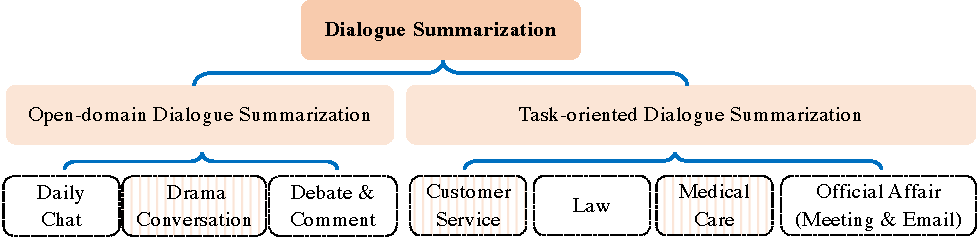
\includegraphics[scale=0.8]{fig/scenarios.pdf}
	\caption{The classification of dialogue summarization tasks with different application scenarios. Datasets proposed for evaluations under each scenario are in Section~\ref{sec:dataset}.}
	\label{fig:scenario}
\end{figure}


We compare and contrast ODS and TDS as follows.
\begin{itemize}
% functional role playing
\item Dialogues happen between \textbf{two or more speakers} both in ODS and TDS, whereas the \textbf{interpersonal relationship} and \textbf{functional relationship} among speakers are different. Generally, speakers in ODS are friends, neighbors, lovers, family members, and so on. 
They are equal either in the aspect of interpersonal relationships or functional relationships. For example, one can raise a question or answer others' questions in online forums~\cite{fabbri2021convosumm}.
In TDS, speakers have different official roles acting for corresponding responsibilities. For example, plaintiff, defendant, witness and judge in court debates~\cite{duan2019legal}, project manager, marketing expert, user interface designer and industrial designer in official meetings~\cite{carletta2005ami} are corresponding roles.
Among different dialogues, roles are the same and can be played by different speakers and a speaker's role is always unchanged for a service platform.
In a word, TDS pays more attention to functional roles while ODS focuses on speakers.


% covering topics
\item Multiple \textbf{topics} may be covered in the same dialogue session.
Topics in ODS are more diverse than in TDS. The summarization models are expected to deal with unlimited open-domain topics such as chitchat, sales, education, and climate at the same time~\cite{chen2021dialsumm}. 
However, topics in TDS are more concentrated and need more expertise for understanding.
Dialogues in TDS either focus on a single domain with more fine-grained topics, such as medical dialogues of different specialties,
or several pre-defined domains, such as restaurant, hotel, and transformation reservation.
Domain knowledge is significant for summarization, and it is divergent across sub-domains. For instance, expertise and medical knowledge are required in doctor-patient dialogues for generating accurate medical concepts~\cite{joshi2020dr} while specific knowledge bases for internal medicine and primary care are not the same.

%  inherent structure
\item The input dialogue for both ODS and TDS is made up of \textbf{a stream of utterance} as defined in Equation~\ref{eq:dialogue}. However, 
the \textbf{structure} of these two types of dialogues are different.
Open-domain dialogues often happen casually and freely while dialogues in TDS may have some inherent working procedures or writing formats. 
For example, the program manager in meetings usually masters the meeting progress~\cite{zhu2020end} implicitly with words such as ``okay, what about ...'', and communications by e-mails consist of semi-structured format including subjects, receivers, senders, and contents~\cite{zhang2021emailsum}. 

% special intentions for summaries
\item \textbf{Focuses of summaries} are distinct. Summaries for ODS in recent research are more like condensed narrative paraphrasing with different levels of granularity. An example is a synopsis from the Fandom wiki\footnote{\url{criticalrole.fandom.com}} maintained by fans for the Critical Role transcripts~\footnote{\url{github.com/RevanthRameshkumar/CRD3}}\cite{rameshkumar2020storytelling}, helping to quickly catch up with what is going on in the long and verbose dialogues. Differently, dialogues in TDS take place with strong intentions for solving problems. Summaries for such dialogues are expected to cover the user intents and corresponding solutions, such as medical summaries for clinical decision making~\cite{joshi2020dr} and customer service summaries for ticket booking~\cite{zhao2021todsum}. As a result, generating faithful content is extremely significant for TDS. %{faithfulness}
\end{itemize}

%\KZ{I feel that just dividing the dialogue summarization into ODS and TDS is a bit
%too coarse-grained. Later when you discuss the approaches, u need to associate
%each approaches with a certain characteristic/scenario of the task. It's more
%useful if u can use some refined characteristics of the task.}

\section{Background and Related Work}
In this section, we present the necessary background knowledge about matrix factorization and unstructured pruning (\figref{fig:intro}).

\begin{figure}[t!]
	\centering
	\scalebox{0.154}{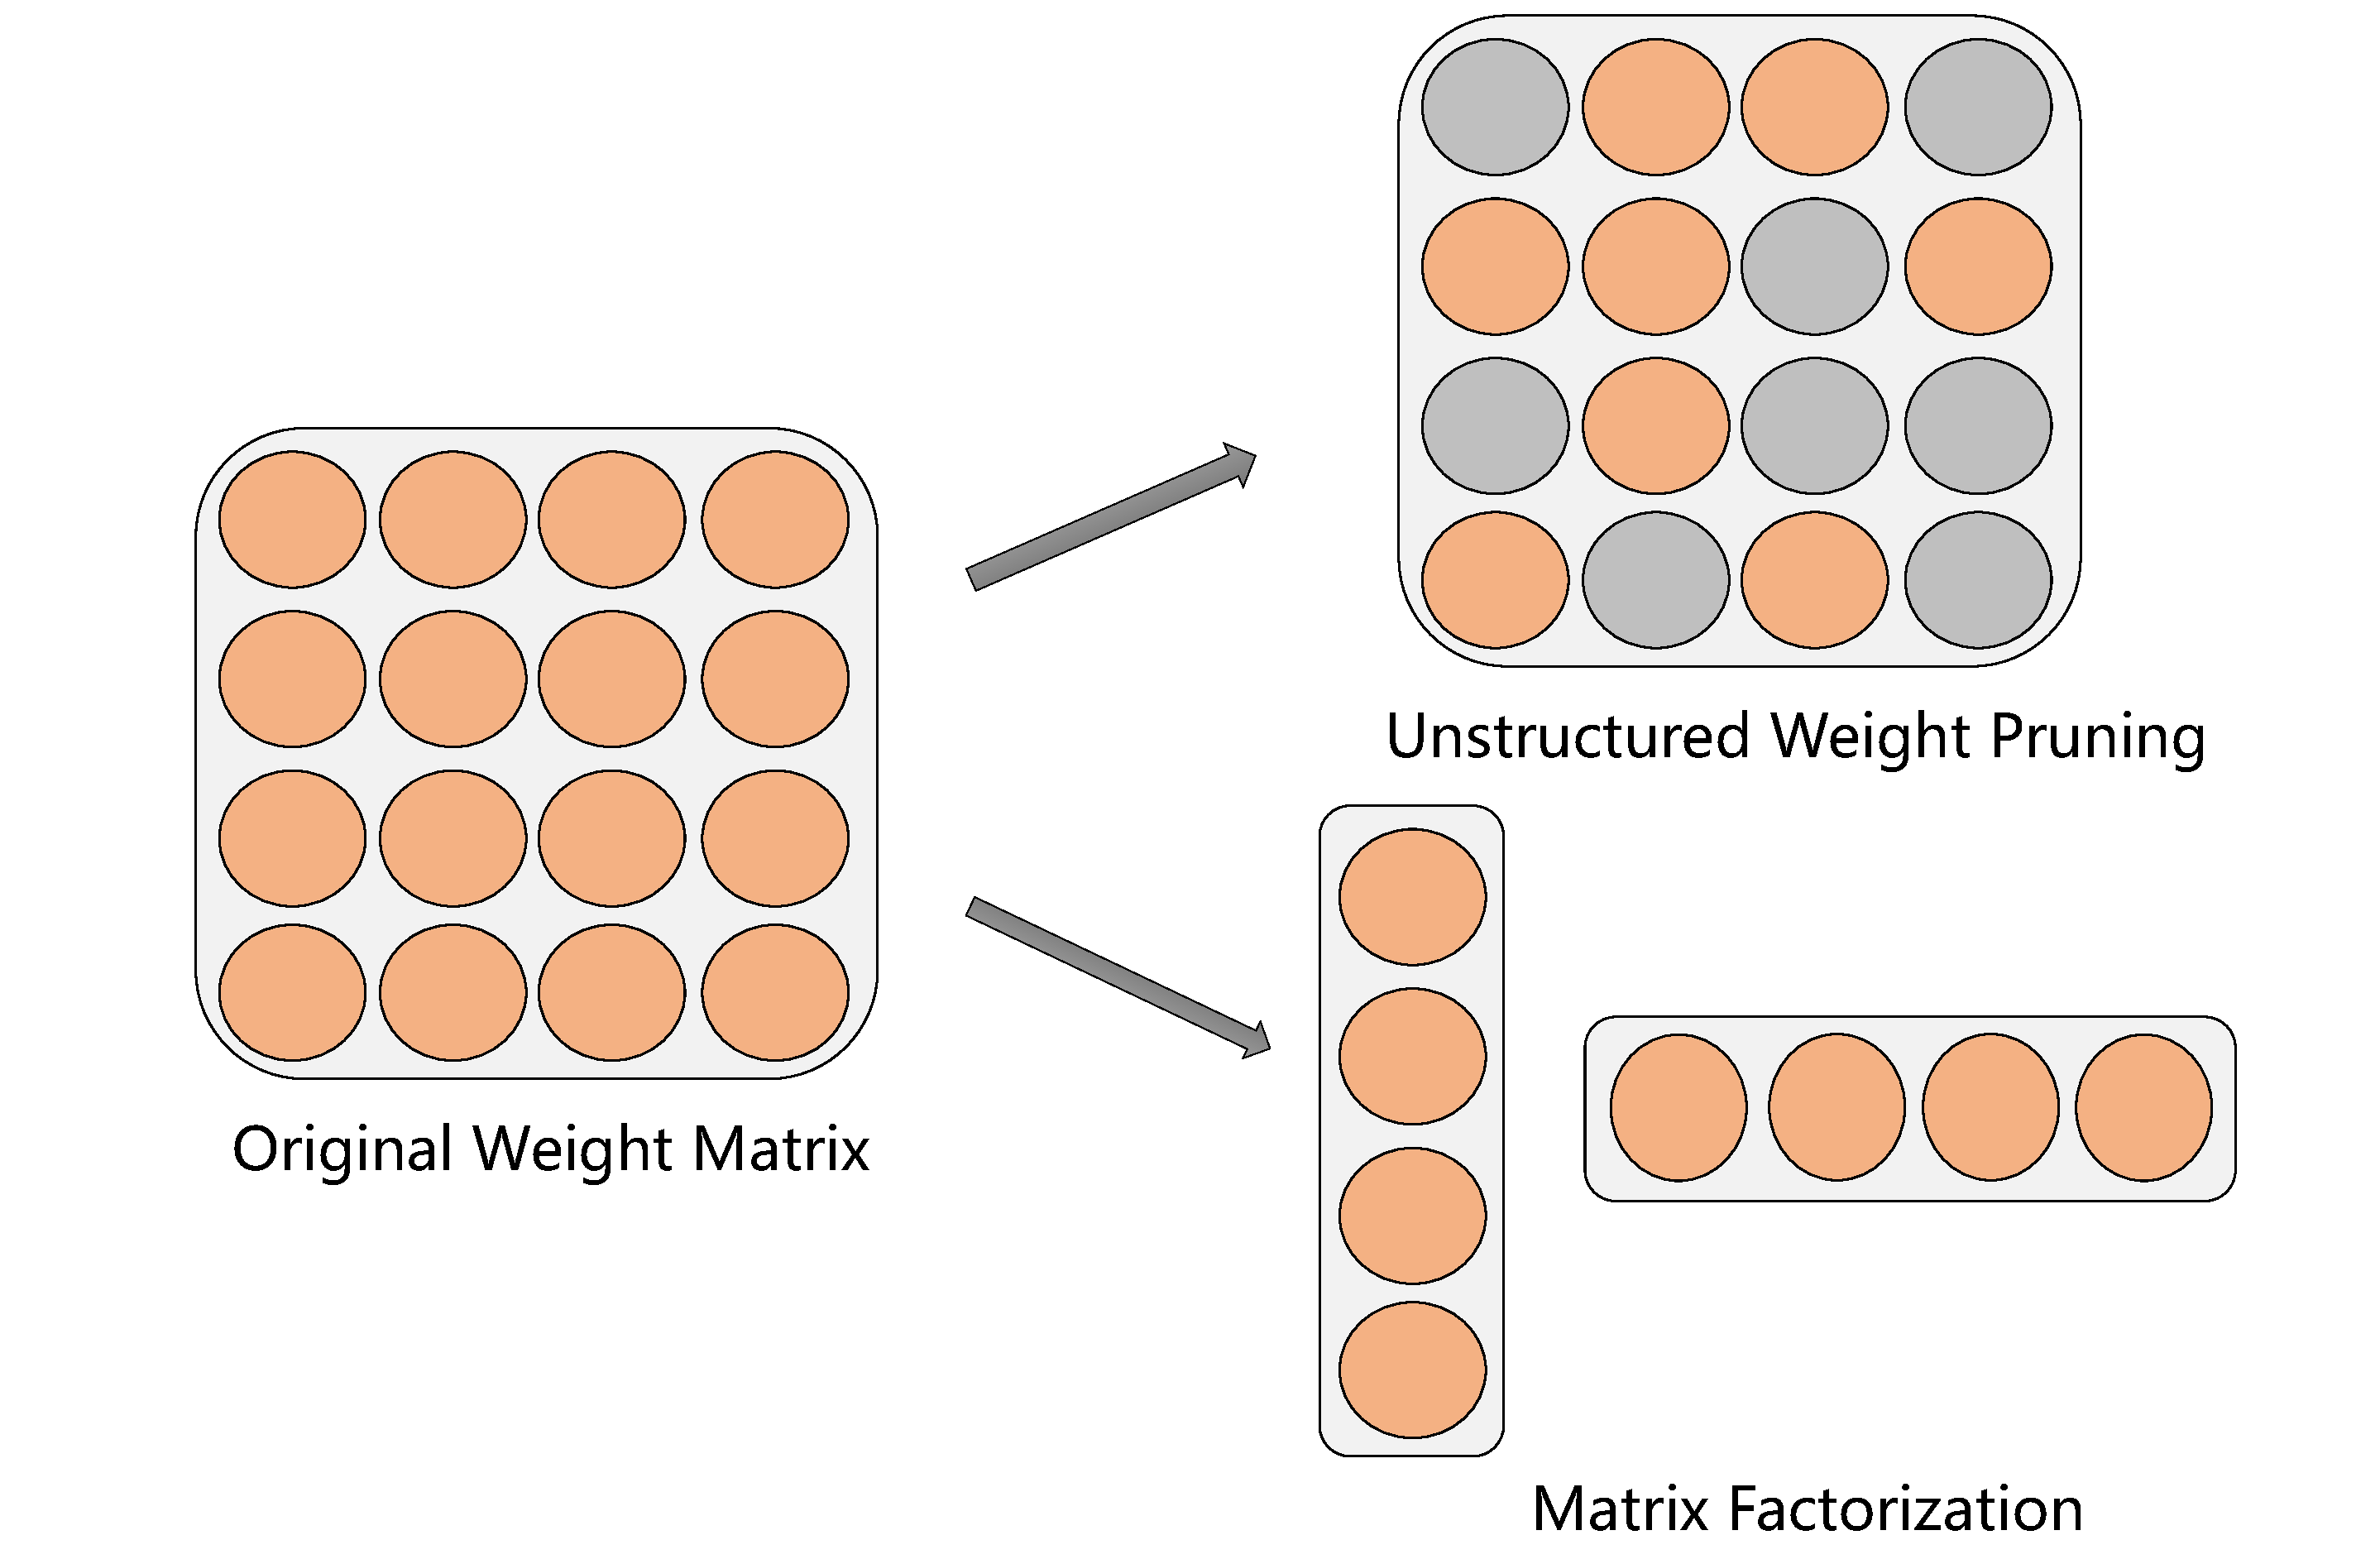
\includegraphics{./figures/intro_final.pdf}}
	\caption{Illustration of matrix factorization and unstructured pruning  on a single weight matrix.}
	\label{fig:intro}
\end{figure}

\subsection{Matrix Factorization~(MF)}
\label{sec:lr}
Given the weight matrix $\bm{W}\in \mathbb{R}^{n\times m}$, matrix factorization~\cite{svd} decomposes it into sub-matrices with reduced total number of parameters to achieve model compression.  
It first uses singular value decomposition~(SVD) to obtain an equivalent 
form of $\bm{W}$ as the product of three matrices:
\begin{align}
	\bm{W}=\bm{U}\bm{\Sigma}\bm{V}^\mathrm{T}
\end{align}
where $\bm{U}\in \mathbb{R}^{n\times r}$, $\bm{\Sigma}\in  \mathbb{R}^{r\times r}$, $\bm{V}\in \mathbb{R}^{r\times m}$, and $r$ is the rank of matrix $\bm{W}$. $\bm{\Sigma}$ is a diagonal matrix of non-zero singular values $\{\sigma_1, \sigma_2,...,\sigma_r\}$ in descending order. Then, low-rank approximation with targeted rank $k$ is obtained by keeping the top-$k$ singular values in $\bm{\Sigma}$ as well as their corresponding column vectors in $\bm{U}$ and $\bm{V}$:
\begin{align}
	\bm{W}&\approx \bm{U}_{[:, :k]}\bm{\Sigma}_{[:k,:k]}\bm{V}_{[:, :k]}^{\mathrm{T}} =\bm{A}\bm{B}
	\label{eq:svd}
\end{align}
where $\bm{A}=\bm{U}_{[:,:k]}\bm{\Sigma}_{[:k,:k]}$ and $\bm{B}=\bm{V}_{[:,:k]}^{\mathrm{T}}$ are the two final sub-matrices of which the product is used to replace $\bm{W}$. After such factorization, the number of parameters is reduced from $nm$ to $k(n+m)$. Different compression rates can be achieved by varying the preserved rank $k$.



\subsection{Unstructured  Pruning~(UP)}
\label{sec:pruning}
%We first establish some shared notations for unstructured weight pruning. 
Let $\bm{W}\in \mathbb{R}^{n\times m}$ denote a generic weight matrix in a PLM. In order to determine which elements in $\bm{W}$ are pruned, an importance score matrix $\bm{S}\in \mathbb{R}^{n\times m}$ is correspondingly introduced. The smaller $S_{i,j}$ is, the larger the probability of $W_{i,j}$ will be pruned. Given the importance scores, a pruning strategy $f_{prune}(\cdot)$ computes a binary mask matrix $\bm{M}\in \{0,1\}^{n\times m}=f_{prune}(\bm{S})$, 
and the forward process for an input $x$ becomes $y=(\bm{W}\odot\bm{M})x$, 
where $\odot$ denotes element-wise multiplication.

\paragraph{Zero-order Pruning~(UP$_{\text{zero}}$)} Zero-order pruning refers to the family of algorithms that only use the value of the weight as the importance measure.
For example, magnitude-based weights pruning~\cite{mag,chen2020lottery} adopts the absolute value of weight as importance score, i.e., 
$\bm{S}_{i, j}=|\bm{W}_{i, j}|$. The typical choice of $f_{prune}(\cdot)$ is to keep $v\%$  of weights with the largest importance scores:
\begin{align}
	\bm{M}_{i,j}=
	\begin{cases} 
		1, & \text{if }\bm{S}_{i,j}~\text{is in the largest }v\%\\
		0,  & \text{otherwise}  
	\end{cases}
	\label{eq:zero}
\end{align}


\paragraph{First-order Pruning~(UP$_\text{first}$)} Unlike zero-order pruning where $\bm{S}$ is directly derived from $\bm{W}$, first-order methods treat 
$\bm{S}$ as learnable parameters and jointly train it with model weights 
during fine-tuning. For example, SMvP~\cite{movement} and CAP~\cite{cap}
randomly initialize $\bm{S}$ and update it during the whole pruning process. The pruning strategy $f_{prune}(\cdot)$ is the same as in zero-order pruning~(\eqnref{eq:zero}).


%\begin{align}
%	\bm{M}_{i,j}=
%	\begin{cases} 
%		1, & \text{if }\bm{S}_{i,j}\ge \tau\\
%		0,  & \text{otherwise}  
%	\end{cases}
%	\label{eq:first}
%\end{align}
Since the gradient of the thresholding function is 0 everywhere, straight-through estimator~\cite{st} is used as an approximation. The importance score $\bm{S}_{i,j}$ of $\bm{W}_{i,j}$ up to training step $T$ can be expressed as: 
\begin{align}
\bm{S}_{i,j}=-\sum_{t\le T}(\frac{\partial \mathcal{L}}{\partial \bm{W}_{i,j}})^{(t)} \bm{W}_{i,j}^{(t)}
\end{align}
where $\mathcal{L}$ is the loss function. The formulation is also equivalent to the first-order Taylor approximation of the change in $\mathcal{L}$ if $\bm{W}_{i,j}$ is zeroed out.

\paragraph{Sparsity Scheduler}
The proportion of remaining weights is controlled by the sparsity scheduler, here  we adopt the commonly used  cubic sparsity schedule to progressively reach target sparsity, i.e., $v_t$ at time step $t$ is derived by:
\begin{align}
	%	v^{(t)}=
	\begin{cases} 
		v_i & t\in [0, t_i) \\
		v_f+(v_i-v_f)(\frac{T-t_{f}-t}{T-t_f-t_i})^3 & t\in[t_i, T-t_f) \\
		v_f  & \text{otherwise}  
	\end{cases}
\end{align}
\label{eq:prune}
where $v_i=1.0$, $v_f$ is the final percent of remained parameters, $t_i$ and $t_f$ are the warmup and cool-down steps. $T$ is the total training steps. Moreover, we discard $\bm{M}$ and directly set $\bm{W}_{i,j}$ to zero if $\bm{S}_{i,j}^{(t)}$ is not in the top-$v_t$ at time step $t$. 
%\paragraph{A Unified View} The differences in the implementation of 
%importance scores~(direct value inspection v.s. additional learnable 
%parameters) and pruning strategy~(top-$v$ selection v.s. tuned threshold) 
%make it hard to compare various pruning methods. To this end, 
%we establish a unified view of zero-order and first-order pruning, 
%denoted as \textbf{UWP$_\text{zero}$} and \textbf{UWP$_\text{first}$}, 
%with the only difference being the calculation of importance score $\bm{S}$.
%\KZ{This section is a little strange here because it seems to repeat
%what has been said in the previous subsections. You have already defined $S$
%but now you are singling out $S$ again. In particular, I can't appreciate why
%``it is hard to compare various pruning methods'', I don't really see
%the need for this unified view.}
%
%For UWP$_\text{zero}$, the calculation of $\bm{S}$ is the same as magnitude pruning, i.e., $\bm{S}_{i, j}^{(t)}=|\bm{W}_{i, j}^{(t)}|$, where $t$ is the time step. For UWP$_\text{first}$, we directly calculate its importance score $\bm{S}$ without introducing additional parameters, i.e.,  $\bm{S}_{i,j}^{(t)}=\bm{S}_{i,j}^{(t-1)}+|\frac{\partial \mathcal{L}}{\partial \bm{W}_{i,j}}^{(t)} \bm{W}_{i,j}^{(t)}|$. 

%\KZ{\eqref{eq:prune} seems 
%to be something new in this section but then it is part of the first-order 
%pruning, and nothing to do with zero-order pruning. So why is it in the 
%``unified view?''}

%\KZ{My feel is that this whole section of related work and background is a bit
%long-winded.}
 


\section{Preliminary Study}
\label{sec:pilot}
In this section, we conduct a preliminary study on unstructured pruning  and matrix factorization
based on BERT-base and try to find answers to the following two questions: (1) How does matrix factorization perform under high compression rates? (2) Do subnetworks produced by unstructured pruning contain \textit{low-rank} sparsity patterns while preserving the majority of task accuracy?
%\KZ{What kind of insight? You stop short of providing the motivation
%of the following experiments. Are you trying to see if these two methods alone
%work well to compress language model?}

\subsection{Experimental Setting}
\indent
\paragraph{Datasets}We use two tasks from GLUE benchmark~\cite{glue}, namely MRPC and RTE, as our evaluation testbeds. Both of them are formulated as classification problems.

\paragraph{Implementation Details} For matrix factorization, we follow the algorithm in \secref{sec:lr}. Specifically, we first fine-tune BERT-base on each downstream task following \citet{bert}. Then, we perform truncated SVD on weight matrices of each linear layer in the fine-tuned BERT and re-train the whole model to recover the lost accuracy. We select preserved rank $k$ from $\{390, 260, 130, 50\}$, which corresponds to $\{0.75, 0.50, 0.25, 0.10\}$ of BERT's parameters.

For unstructured  pruning, we evaluate both UP$_\text{zero}$ and UP$_\text{first}$. We set the value of $v_f$ from $\{0.75, 0.50, 0.25, 0.10\}$ to make a direct comparison to matrix factorization.

\subsection{Results and Analysis}
\label{sec:pilot_results}

%\begin{figure*}[t]
%	\centering
%	\scalebox{0.285}{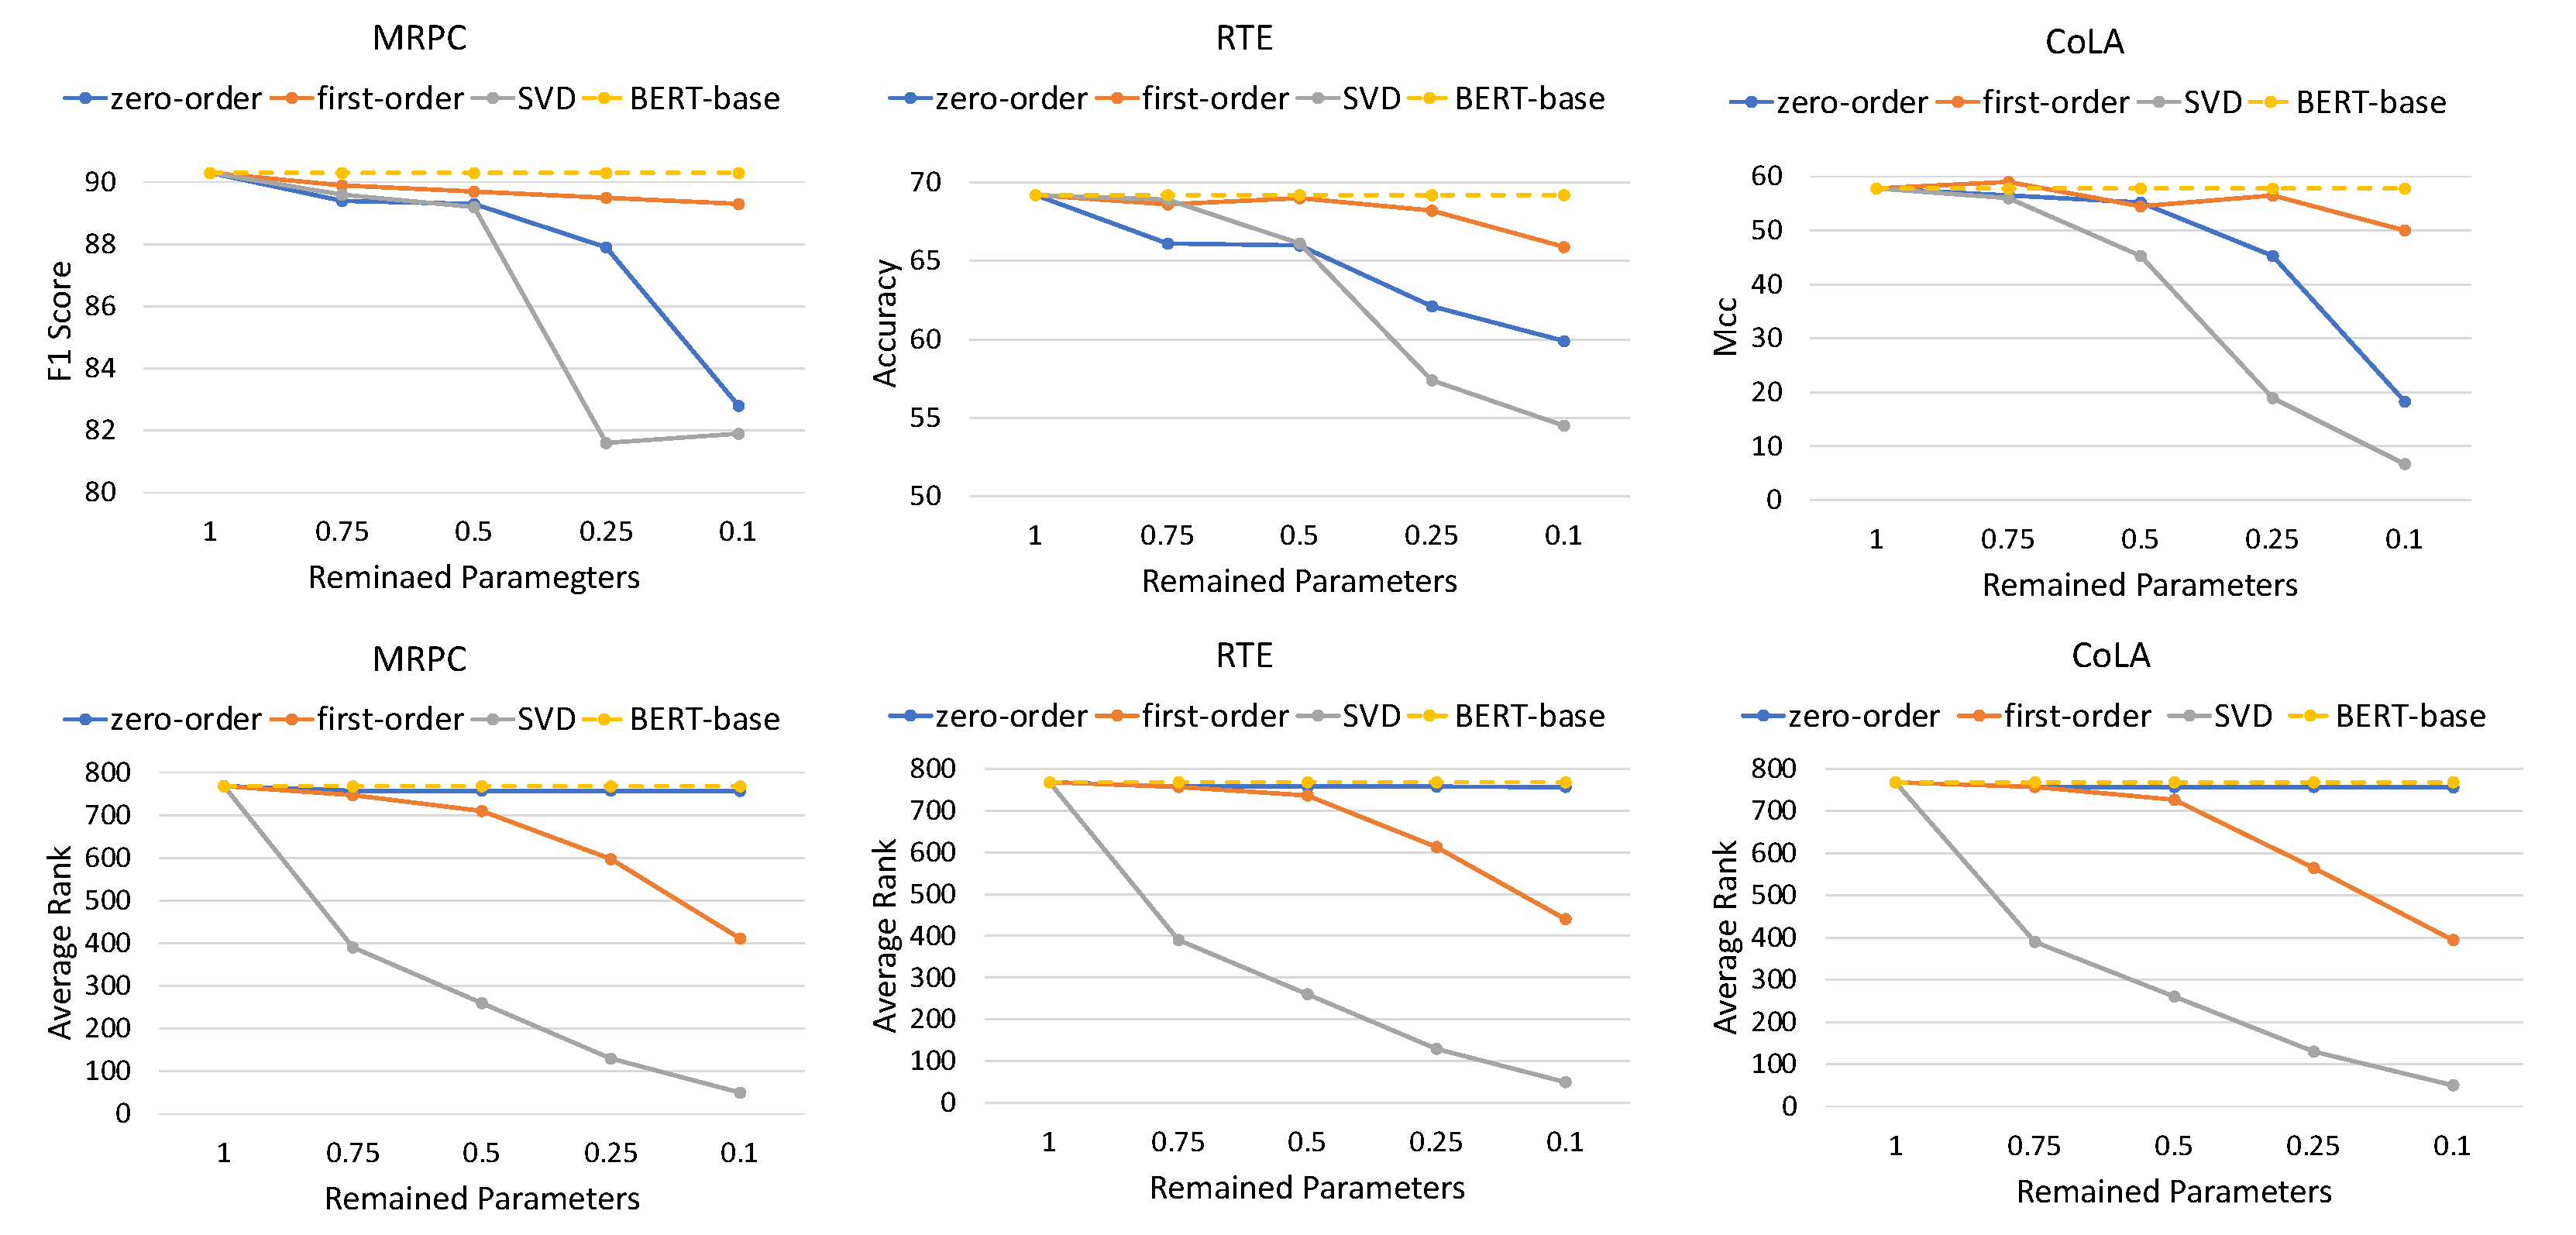
\includegraphics{./figures/pre_new.pdf}}
%	\caption{Task performance~(top half) and average matrix rank~(bottom half) v.s. percent of remained parameters. The dashed yellow line indicates the performance/rank upper bound by fine-tuning the full-scale BERT-base model.}
%	\label{fig:pre}
%\end{figure*}


\paragraph{Accuracy Preservation} 
The variation of task accuracy with respect to the remaining parameters is illustrated 
in the top half of \figref{fig:pre}. Under a small compression rate, i.e., 
$75\%$  parameters remaining, all examined methods can retain $\ge 97\%$ performance 
of BERT-base across all tasks. Under moderate compression rate, i.e., $50\%$ parameters remaining, UP$_\text{zero}$ and SVD start to show obvious declines. 
When more extreme compression rates are pursued, e.g., $25\%$-$10\%$ parameters 
remaining, SVD exhibits the most drastic performance drops compared to UP methods. 
On the contrary,  UP$_\text{first}$ still retains $\sim 97.6\%$ of BERT's performance.
UP$_\text{zero}$ lags behind UP$_\text{first}$ by a large margin under high sparsity. This indicates that magnitude alone cannot be used to quantify a weight's 
contribution because even a small weight can yield a huge influence on the model 
output due to the complicated compositional nature of neural networks. 
In contrast, the importance criterion of UP$_\text{first}$ directly reflects the 
sensitivity of the model's training loss w.r.t. each weight and is therefore more 
accurate.

\begin{figure}[t]
	\centering
	\scalebox{0.175}{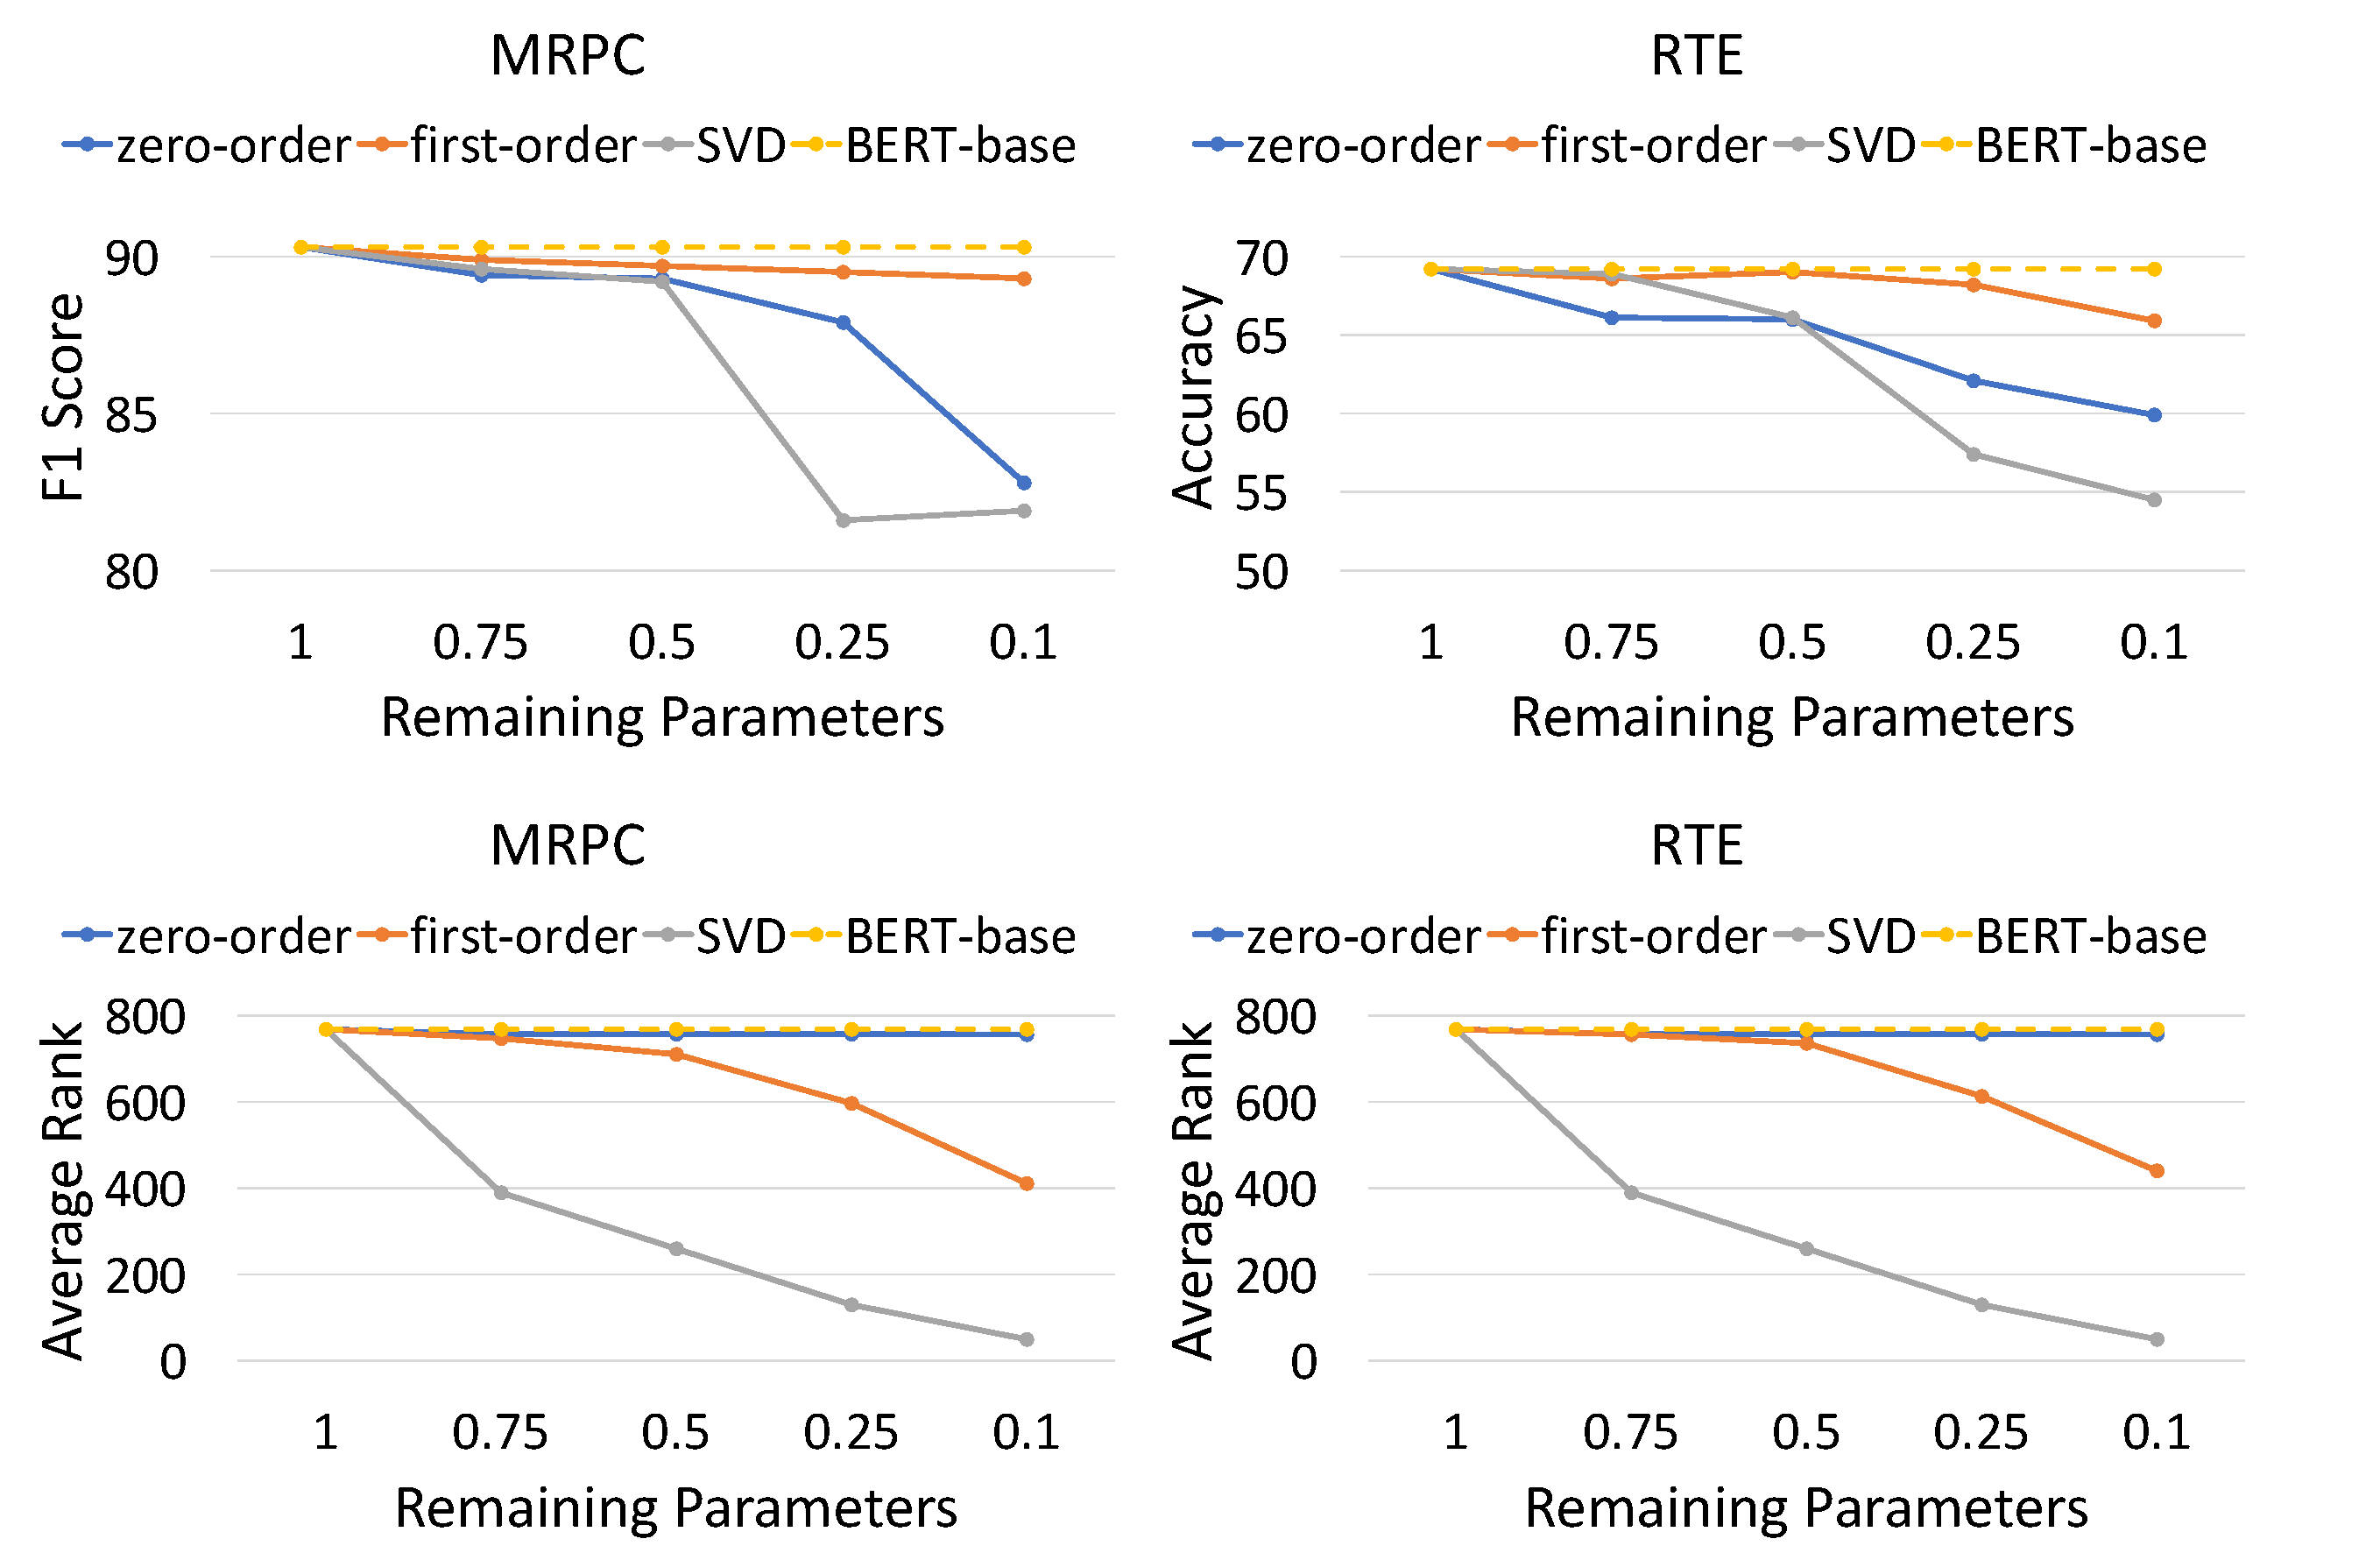
\includegraphics{./figures/pre_col.pdf}}
	\caption{Task accuracy~(top half) and average matrix rank~(bottom half) 
v.s. percentage of original parameters retained. 
The dashed line indicates the performance/rank upper bound by fine-tuning the full-scale BERT-base model. Results on more datasets are deferred to Appendix \ref{sec:A}.}
	\label{fig:pre}
\end{figure}

\begin{figure}[t]
	\centering
%	\scalebox{0.50}{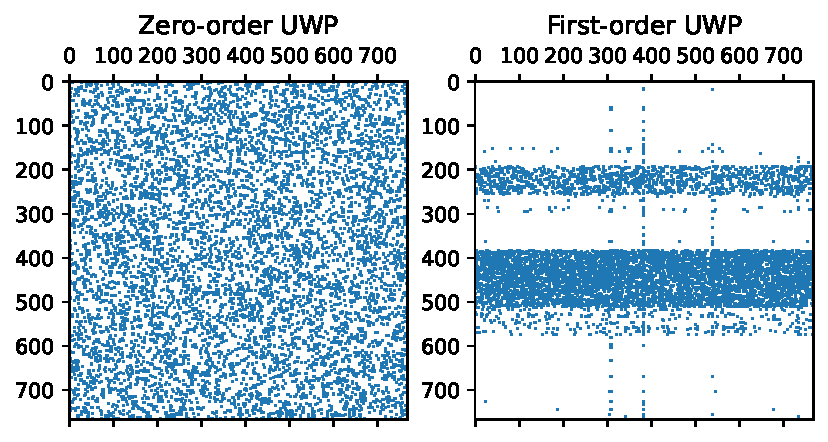
\includegraphics{./figures/sparsity_pattern.pdf}}
		\scalebox{0.50}{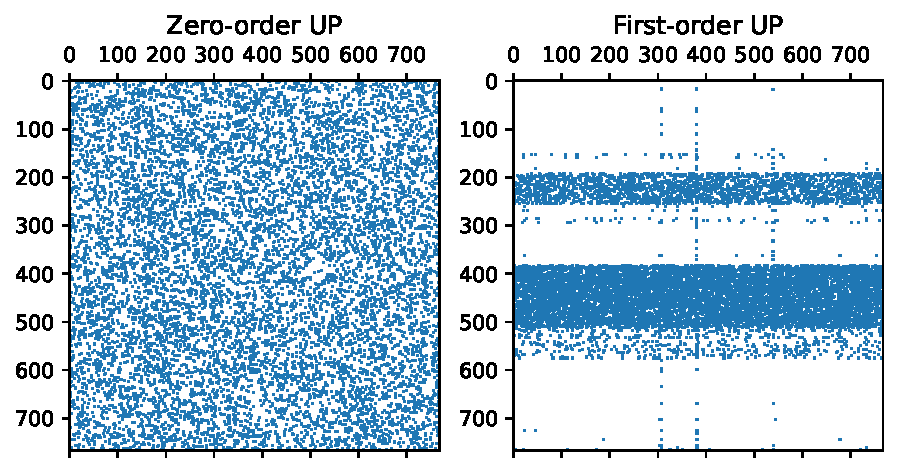
\includegraphics{./figures/zero_first_UP.pdf}}
	\caption{Sparsity patterns of the same 768x768 weight matrix  pruned by UP$_\text{zero}$~(left) and UP$_\text{first}$~(right) on MRPC with $10\%$ of
the parameters remaining.}
	\label{fig:pattern}
\end{figure}

\paragraph{Rank} 
Considering the inferior accuracy of SVD, we hypothesize that the weight matrices of fine-tuned BERT are high-rank, 
hence leading to a large approximation error when $k$ is small. The bottom half of \figref{fig:pre} inspects the average rank of weight matrices. We can see that the weight matrices in fine-tuned BERT-base are nearly full-rank, which explains the inefficacy of SVD when $k$ is small. We also plot the rank-parameter curve of UP methods. For UP$_\text{zero}$, it produces sparse matrices that are 
as high-rank as densely fine-tuned BERT even when $90\%$ weights are set to zero. In contrast, UP$_\text{first}$  produces sparse patterns whose rank monotonically decreases as more weights are pruned. To gain more insights into this phenomenon, we visualize the weight matrix pruned by UP$_\text{zero}$ and UP$_\text{first}$ in \figref{fig:pattern}. Though both are designed without structural bias,  unlike UP$_\text{zero}$, UP$_\text{first}$ learns to remove entire rows from the weight matrix and 
the resulting matrix enjoys a low-rank characteristic.



\begin{figure}[th]
	\centering
	\scalebox{0.142}{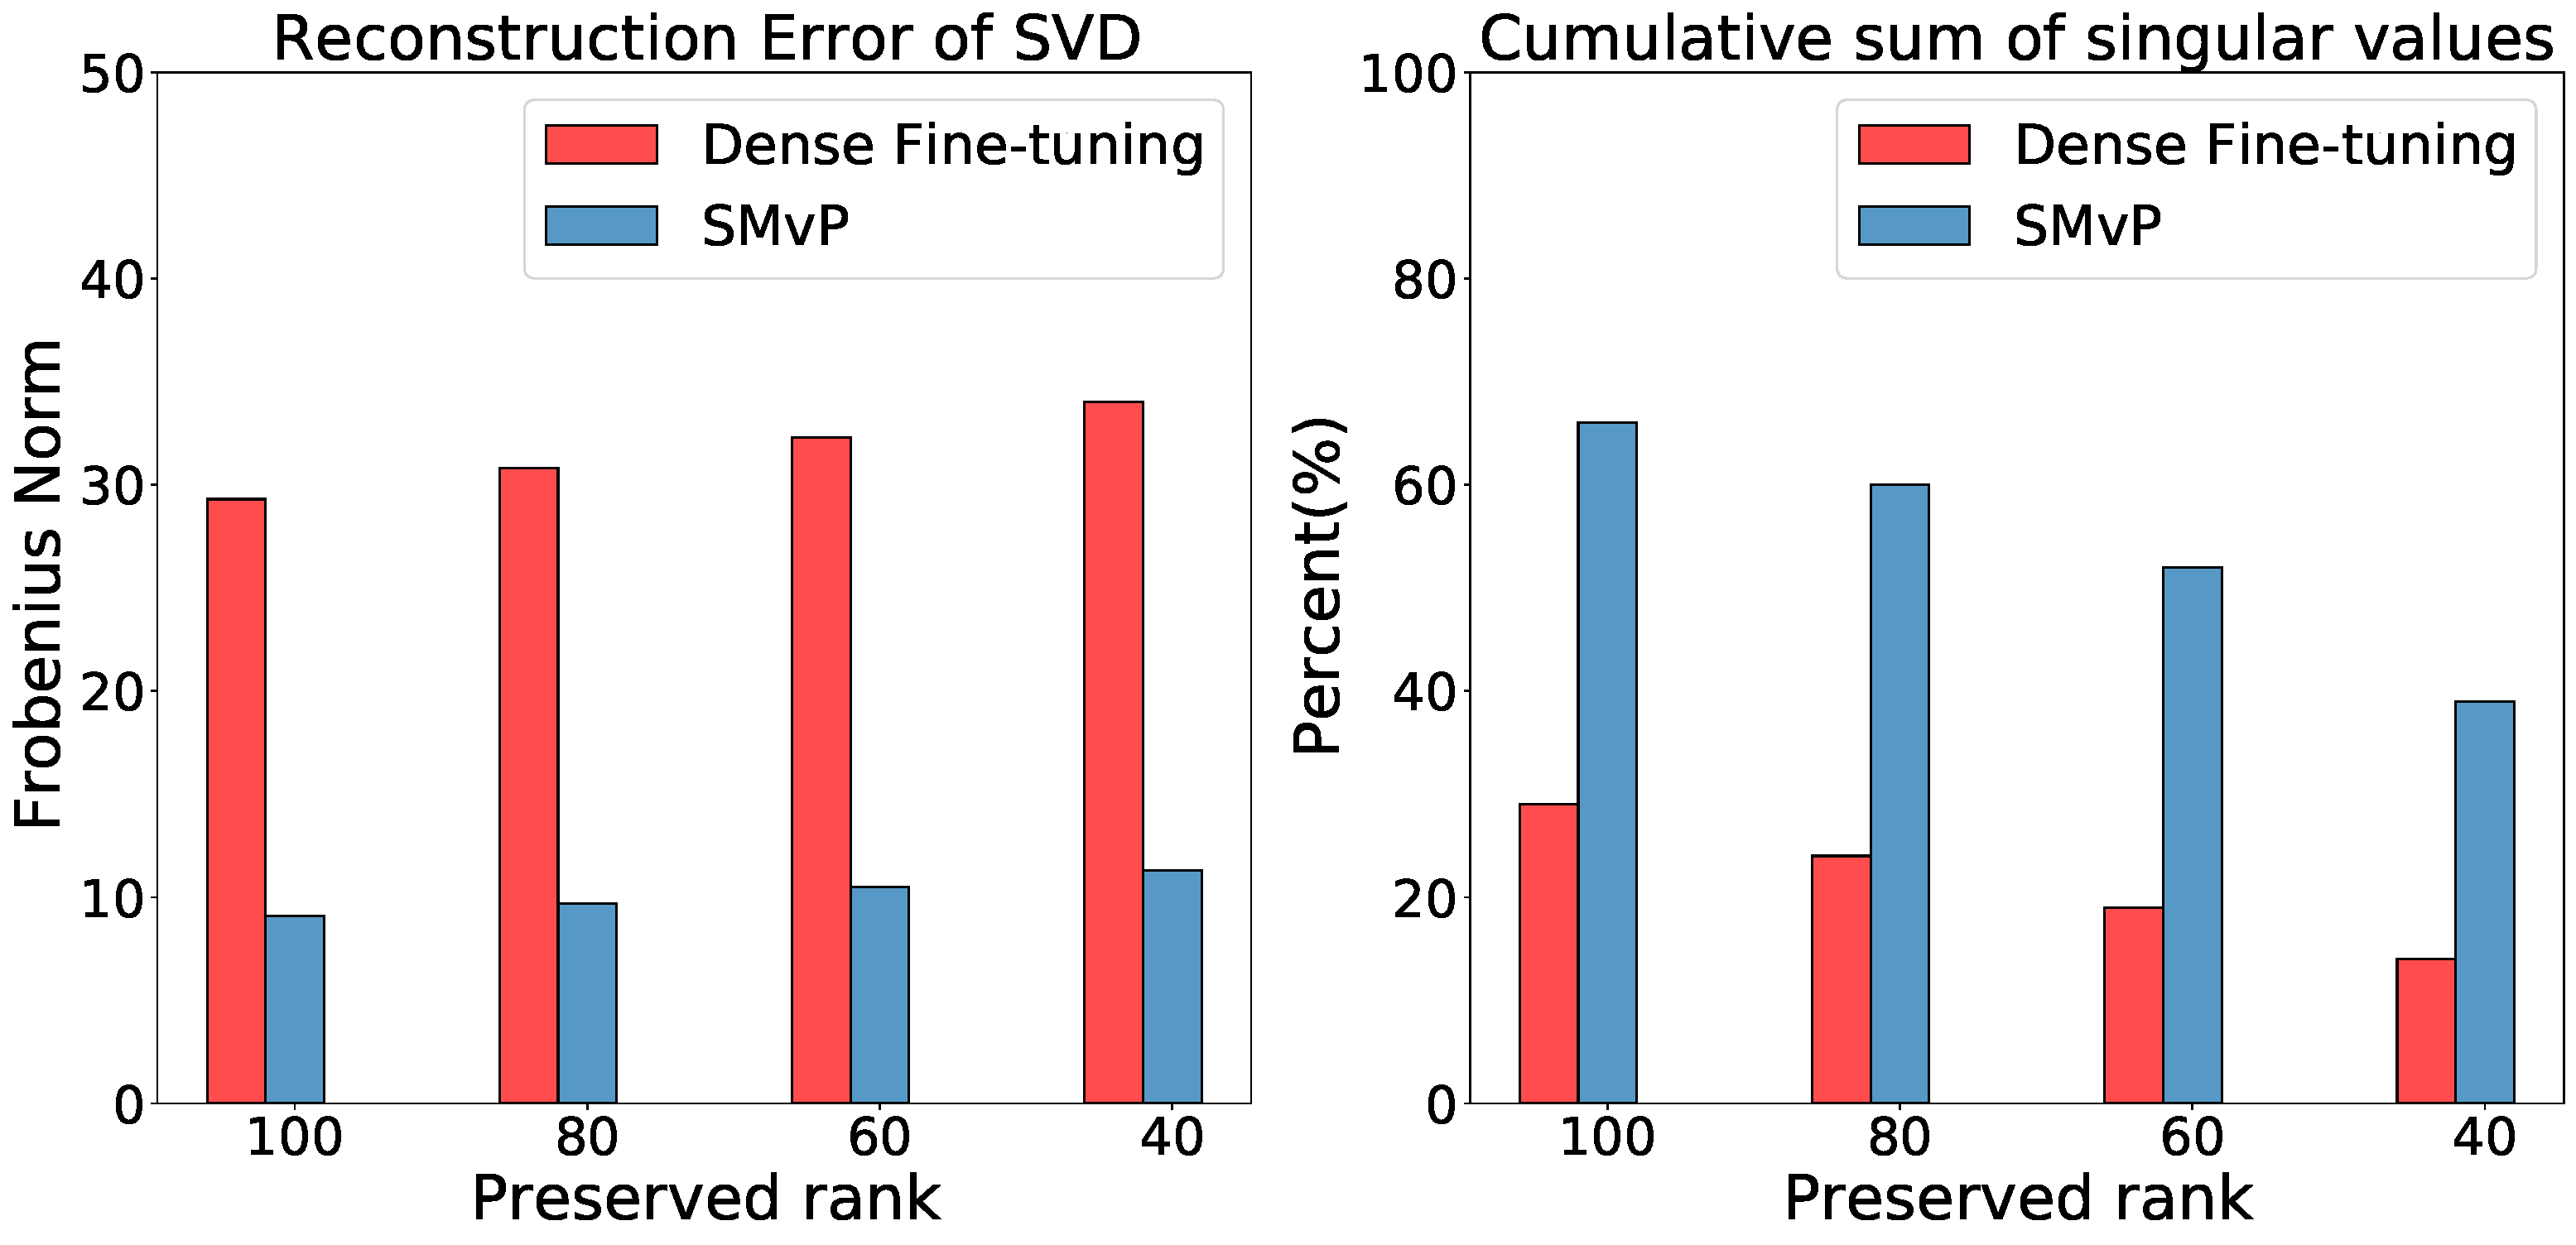
\includegraphics{./figures/norm_vis.pdf}}
	\caption{Quantitatively measuring approximation quality via reconstruction error~(left) and cumulative sum of singular values~(right) on MRPC.}
	\label{fig:norm}
\end{figure}

\paragraph{The Idea}
%\KZ{The key insight is: factorize a high-rank matrix into low rank sub-matrices
%loses a lot of info, but factorize a low-rank matrix into low rank sub-matrices
%doesn't lose as much info. Our design is based on this insight. I think as long
%as you make this insight clear, that's good enough. Some of this section
%is a bit verbose.} 
%Given the fact that factorizing from a low-rank matrix into sub-matrices loses less information than factorizing from a high-rank matrix
%Given the competitive task performance and low-rank structure of UWP$_\text{first}$, 
%it appears plausible to perform low-rank matrix factorization on 
%low-rank sparse models for model compression. 
The key insight is: factorizing a high-rank matrix into low rank sub-matrices
loses significant quantity of useful information, but factorizing a low-rank matrix into low rank sub-matrices
doesn't lose as much information. Our design is based on this insight. 
As a sanity check of its feasibility, we quantitatively measure the 
quality of low-rank approximation with various preserved ranks $k$. 
\figref{fig:norm} shows that given a specific $k$, 
the sum of top-$k$ singular values of matrices produced by UP$_\text{first}$ takes a much larger portion of total values than fine-tuning, suggesting that we can reserve more information of low-rank sparse matrix given the same $k$. The reconstruction error~(measured by Frobenius norm) of UP$_\text{first}$ is also significantly lower, implying a higher approximation quality. We thus expect that low-rank matrix factorization on low-rank sparse models to effectively combine: 
(1) the good performance of first-order UP; 
(2) direct memory and computation reduction by MF.

\section{LPAF: Low-rank Prune-And-Factorize}
\label{sec:approach}
Here we formally propose the LPAF~(\textbf{L}ow-rank \textbf{P}rune-\textbf{A}nd-\textbf{F}actorize) framework 
for language model compression. In addition, 
we propose two optimizations in the 
initialization and training of the compression process.

\subsection{The Overall Workflow}
\label{sec:ptf}
Given a pre-trained language model $T$ and a downstream task with training set $D=\{(x_i, y_i), i=1,2,...M\}$, LPAF consists of three steps to realize model compression: 
\begin{itemize}
	\item Step-1: obtaining the low-rank sparse model $T_{\text{sparse}}=\text{UP}_\text{first}(T,D, v)$. $v$ is the percent of remained parameters after pruning.
	\item Step-2:  performing matrix factorization on each weight matrix~(excluding the embedding layer) in $T_{\text{sparse}}$ and  obtain its low-rank factorized form $T_{\text{factorized}}$. 
	%	The perceivable reduction of model's memory footprint and computation cost happens at this step.
	\item Step-3:  re-training $T_{\text{factorized}}$ on $D$ using task-specific loss function until convergence. 
	%	Since step 2 inevitably loses certain task-specific information, this step is designed to ensure that the compressed model retain good task performance.
\end{itemize}

Next, we present two novel optimizations, namely \textit{sparsity-aware SVD} and \textit{mixed-rank fine-tuning}, that improves the matrix factorization and fine-tuning process in step 2 and step 3 respectively.

\subsection{Optimization 1: Sparsity-aware SVD}
\label{sec:sasvd}
SVD has been shown~\cite{bestsvd} to provide the optimal rank-$k$ approximation to $\bm{W}$ with respect to the Frobenius norm:
\begin{align}
	\nonumber
	\min_{\bm{A},\bm{B}} ||\bm{W}-&\bm{A}\bm{B}||_{F}=\min_{\bm{A},\bm{B}} \sum_{i,j}(\bm{W}_{i,j}-(\bm{AB})_{i,j})^2 \\
	& \text{s.t.}~~~~\text{rank}(\bm{AB})=k
\end{align}
It is a generic factorization method in that it is applicable to any matrix $\bm{W}$ by penalizing the reconstruction error of each individual weight equally. 

In our case, $\bm{W}$ is a sparse matrix from $T_{\text{sparse}}$ in which the majority of weights are set to zero by the pruning algorithm $P$. These zero weights are deemed to have less impact on the task performance compared to the retained~(unpruned) weights. However, the vanilla SVD treats each weight equally without considering the inherent sparseness of $W$, thus may be sub-optimal for preserving useful information in $W$ about the end task.
To address this issue, we propose sparsity-aware SVD which considers different priorities of parameters and weighs the individual reconstruction error based on its importance score $\bm{S}_{i,j}$:
\begin{align}
	\min_{\bm{A},\bm{B}} \sum_{i,j}&\bm{S}_{i,j}(\bm{W}_{i,j}-(\bm{AB})_{i,j})^2~~~\\\
	 & \text{s.t.}~~\text{rank}(\bm{AB})=k
	\label{eq:sasvd}
\end{align}
In this way, parameters that are more important can be better reconstructed, hence retaining more task performance from $T_{\text{sparse}}$ at initialization. Nevertheless, \eqnref{eq:sasvd} does not have a closed form solution~\cite{weightedsvd,hsu2021language} when each $\bm{W}_{i,j}$ has its own weight. We therefore resort to a simplification by letting the same row of $\bm{W}$ share the same importance. The importance for row $i$ is given by $\hat{\bm{S}}_{i}=\frac{\sum_{j}\bm{S}_{i,j}}{\sum_{n}\hat{\bm{S}}_{n}}$. Let $\hat{\bm{I}}=diag(\hat{\bm{S}}_1,\hat{\bm{S}}_2,...,\hat{\bm{S}}_{n})$ denote a diagonal matrix,  \eqnref{eq:sasvd} is now converted to:
\begin{align}
	&\min_{\bm{A},\bm{B}}||\hat{\bm{I}}\bm{W}-\hat{\bm{I}}\bm{A}\bm{B}||_F~~~~
	\\
	& \text{s.t.}~~\text{rank}(\bm{AB})=k
\end{align}
This essentially amounts to applying rank-$k$ SVD upon $\hat{\bm{I}}\bm{W}$, i.e., $\hat{\bm{I}}\bm{W}=\hat{\bm{U}}\hat{\bm{\Sigma}}\hat{\bm{V}}^\mathrm{T}$. Then the solution of $\bm{A}$ and $\bm{B}$ can be analytically obtained by:
\begin{align}
	\bm{A} &= \hat{\bm{I}}^{-1}\hat{\bm{U}}_{[:,:k]}\hat{\bm{\Sigma}}_{[:k,:k]},\bm{B}=\hat{\bm{V}}_{[:,:k]}^{\mathrm{T}}
\end{align}


\subsection{Optimization 2: Mixed-rank Fine-tuning}
Recall that the last step of LPAF is to fine-tune $T_{\text{factorized}}$ on the training set $D$. This process has been proven essential to regain the performance lost during factorization~\cite{svd}. However, during the experiments, we observe the performance of fine-tuned $T_{\text{factorized}}$ still slightly lags behind $T_{\text{sparse}}$ given a similar parameter budget. 
%\KZ{Isn't it normal for $T_{factorize}$ to lag behind $T_{sparse}$? Is there any evidence (experimental results) to show
%this ``lagging''?  Even in Fig. 3, in most cases, $T_{sparse}$ is still better Ours. 
%So I don't see enough motivation for this Mixed-rank fine-tuning.} 
We posit that, due to the reduced capacity~(less trainable parameters) and model-level approximation error incurred by low-rank factorization, joint fine-tuning of low-rank matrices may converge to sub-optimal solutions with lower generalization ability. To mitigate this problem, we propose mixed-rank fine-tuning, a regularized scheme for training low-rank matrices.

Let $\{(\bm{A}\bm{B})_i, i=1,2...,N\}$ denotes all low-rank matrices in $T_{\text{factorized}}$. During training, for each $(\bm{A}\bm{B})_i$, we sample a binary Bernoulli random variable $z_i\sim \text{Bernoulli}(p)$, where $p$ is a global hyper-parameter. Then, the local computation process involving $(\bm{A}\bm{B})_i$ is modified to:
\begin{align}
	\bm{x}_{out} = (1-z_i)*(\bm{A}\bm{B})_i \bm{x}_{in} + z_i * \bm{W}_i\bm{x}_{in} 
\end{align}
where $\bm{W}_i$ is the sparse matrix in $T_{\text{sparse}}$ from which $\bm{A}_i$ and $\bm{B}_i$ are derived. In this way, the low-rank matrices can further 
benefit from gradient-level regularization from  $T_{\text{sparse}}$, 
thus reducing the generalization gap. The hyper-parameter $p$ is controlled by a scheduler. We implement it such that $p$ is linearly decayed from an initial value $p_{\text{init}}$ to zero by a constant step size $d$:
\begin{align}
	p = \text{max}(0, p_{\text{init}}-d*t)
\end{align}
As $p$ decreases, $\bm{W}_i$ is gradually substituted by low-rank sub-matrices $(\bm{AB})_i$. When $p$ reaches zero, the training enters the phase of standard fine-tuning. To further mitigate the training instability brought by sampling, we let each input go through the forward pass twice with different $\bm{z}^1=\{z_i^1\}_{i=1}^{N}$ and $\bm{z}^2=\{z_i^2\}_{i=1}^{N}$, and impose a consistency objective on the two outputs to promote stability:

\begin{align}
	\mathcal{L}_{c}=\mathcal{D}(y_{\bm{z}^1}, y_{\bm{z}^2})
\end{align}
where $\mathcal{D}$ can be the KL divergence for classification tasks and the MSE loss for regression tasks.

% After $p$ reaches zero, the model still benefits from the regularization effect brought by different dropout masks~\cite{rdrop}.

\section{Experiment Evaluation}
\label{sec:experiment}
In this section, we first give some statistics of our corpus and evaluate the quality and quantity of the learned rules. Then, we compare with other causal knowledge bases. Next, we analyze and discuss some main sub-modules in the rule learning framework. Finally, a practical application of futures price prediction and demonstration are introduced. Our experiments are implemented in Python and SWI-Prolog\footnote{ \url{ http://www.swi-prolog.org/}}.
% and run on a computer with Intel Xeon 32 CPU(2.60GHz) and 173GB memory.
	
\subsection{Dataset}
We crawled the text dataset from Chinese financial news website \footnote{\url{ http://finance.sina.com.cn}}. The news data containing 4,991,000 articles, from 2000/7/20 to 2017/12/31, is used to rule learning.
%	, which are split into \textbf{111,330,205} sentences. The number of unique sentences is \textbf{75,572,053}, covering  \textbf{67.88\%} of the total sentences. 
The number of sentences with causal cue words is 7,147,141, accounting for 9.46\% of the total number of de-duplicated sentences (75,572,053. The repetition rate of sentences is about 32\%).
It shows that about  \textbf{14.2\%} (9.64\%/(1-32\%)) sentences explicitly express causality in online financial news sentences.
The news data containing 270,562 articles, from 2018/1/1 to 2018/11/2, is used to evaluate our framework. We set $\alpha$ to 0.5 to achieve an equal balance between generalization and specialization in rule induction. 
We set $\gamma$ to 0.3 to control the Prolog engine to reason around two steps, since more than two steps lead to obviously unreasonable results.

%	\begin{table}[]
%		\caption{Dataset Information}
%		\begin{center}
%		\begin{tabular}{|l|l|l|}
%			\hline
%			Dataset       & Train & Test \\ \hline
%			Time Interval &       &      \\ \hline
%			Number        &       &      \\ \hline
%		\end{tabular}
%	\end{center}
%	\end{table}

\subsection{Rule Evaluation}
We evaluate these rules both quantitatively and qualitatively.
\paragraph{Quantitative Evaluation}
The number of the final rules we learned is \textbf{50000}. We divide the rule quality into three levels: good, fair and bad. According to the ranking of rule confidence, we randomly select 200 rules from the top 10000 rules and manually divide them into three levels. The `good', `fair', and `bad' levels of them account for \textbf{32.5\%}, \textbf{39.0\%} and \textbf{28.5\%}, respectively.
%	\begin{table}[]
%		\centering
%		\begin{tabular}{|l|l|l|} \hline
%		 good & fair &bad \\ \hline
%			65/200(32.5\%)& 78/200(39.0\%) & 57/200(28.5\%) \\ \hline
%		\end{tabular}
%		\caption{Rule Quality}
%		\label{tab:rule_quality}
%	\end{table}

\paragraph{Qualitative Evaluation}
%\begin{align*}
%%	good
%%	{"c": ["过剩_1", "X_燃料", "产量", "", ""], "e": ["下降_1", "X_自然资源", "价格", "", ""], "relation": [["c_sc", "e_sc", "madeof"]], "ctx": {"senids": [1975666], "pattern_ids": [8]}, "ruleid": 5131, "confidence": 0.5657637042081998}
%&\text{1 (X, '产量/yield', '过剩/surplus', '', ''):-(Y, '价格/price', '下降/fall',} \nonumber\\
%&\text{'',''), IsA(X, '燃料/fuel'), IsA(Y, '自然资源/natural resource'),} \nonumber\\
%&\text{madeof(X, Y)} \\
%%{"c": ["结束_1", "X_国家", "罢工", "", ""], "e": ["下降_1", "X_金属", "价格", "", ""], "relation": [["e_sc", "c_sc", "atlocation"]], "ctx": {"senids": [341012], "pattern_ids": [6]}, "ruleid": 11607, "confidence": 0.5824045924950126}
%&\text{2 (X, '罢工/strike', '结束/stop', '', ''):-(Y, '价格/price', '下降/fall', }\nonumber\\
%&\text{'',''), IsA(X, '国家/nation'), IsA(Y, '金属/metal')}\nonumber\\
%&\text{, atlocation(Y, X)}	 \\
%%{"c": ["下降_1", "X_作物", "价格", "", ""], "e": ["减少_1", "", "", "X_作物", "面积"], "relation": [["c_sc", "e_oc", "=="]], "ctx": {"senids": [961411], "pattern_ids": [8]}, "ruleid": 978, "confidence": 0.5876590112986869}
%&\text{3 (X, '价格/price', '下降/fall', '', ''):-(X, '面积/area', '减少/fall', }\nonumber\\
%&\text{'',''), IsA(X, '作物/crop')} \\
%%fair
%%2{"c": ["下降_1", "X_国家", "储蓄率", "", ""], "e": ["下降_1", "X_国家", "增长率", "", ""], "relation": [["c_sc", "e_sc", "=="]], "ctx": {"senids": [1640122], "pattern_ids": [5]}, "ruleid": 213, "confidence": 0.7185889172176277}
%&\text{4 (X, '储蓄率/saving rate', '下降/fall', '', ''):-(X, '增长率/growth rate', }\nonumber\\
%&\text{'下降/fall','',''), IsA(X, '国家/nation')} \\
%%2{"c": ["下降_1", "", "X_产品", "", ""], "e": ["适合_1", "", "X_作物", "", ""], "relation": [["c_s", "e_s", "madeof"]], "ctx": {"senids": [1791763], "pattern_ids": [6]}, "ruleid": 19783, "confidence": 0.5634539402859007}
%&\text{5 ('', X, '下降/fall', '', ''):-('', Y, '适合/fit', '', ''), IsA(X, }\nonumber\\
%&\text{'产品/product'), IsA(Y, '作物/crop'), madeof(X, Y)}   \\
%%bad
%%1{"c": ["减少_1", "", "X_国家", "X_自然资源", "依赖性"], "e": ["增加_1", "", "", "X_燃料", "销量"], "relation": [["e_oc", "c_oc", "madeof"]], "ctx": {"senids": [1707156], "pattern_ids": [8]}, "ruleid": 4468, "confidence": 0.5717182258485046}
%%另一方面,由于日本、韩国和中国减少对中东地区进口原油的依赖性,道达尔公司希望增加对这三个国家的液化天然气销量。
%&\text{6 ('', X, '减少/fall', Y, '依赖性/dependence'):-('', '', '增加/increase',}\nonumber\\
%&\text{ Z,'销量/sales'), IsA(X, '国家/nation'), IsA(Y, '自然资源/natural-} \nonumber\\
%&\text{resource'), IsA(Z, '燃料/fuel'), madeof(Z,Y)}	
%\end{align*}
Figure \ref{fig:rules_case} shows some typical rules: 1,2,3 are good, 4,5 are fair, and 6 is bad.
The main problems of these rules include:
The extracted events are not incomplete, which makes the rules less informative, such as rule 4 and 5.
The causality between cause event and effect event is not very strong, which should be attributed to the design of causal patterns and the process of rule induction, such as 4 and 6.
Some other problems also exist, such as verb disambiguation when normalizing predicates, noun disambiguation when generalizing rule instances.
%	\begin{figure}[htbp]
%	\begin{center}
%		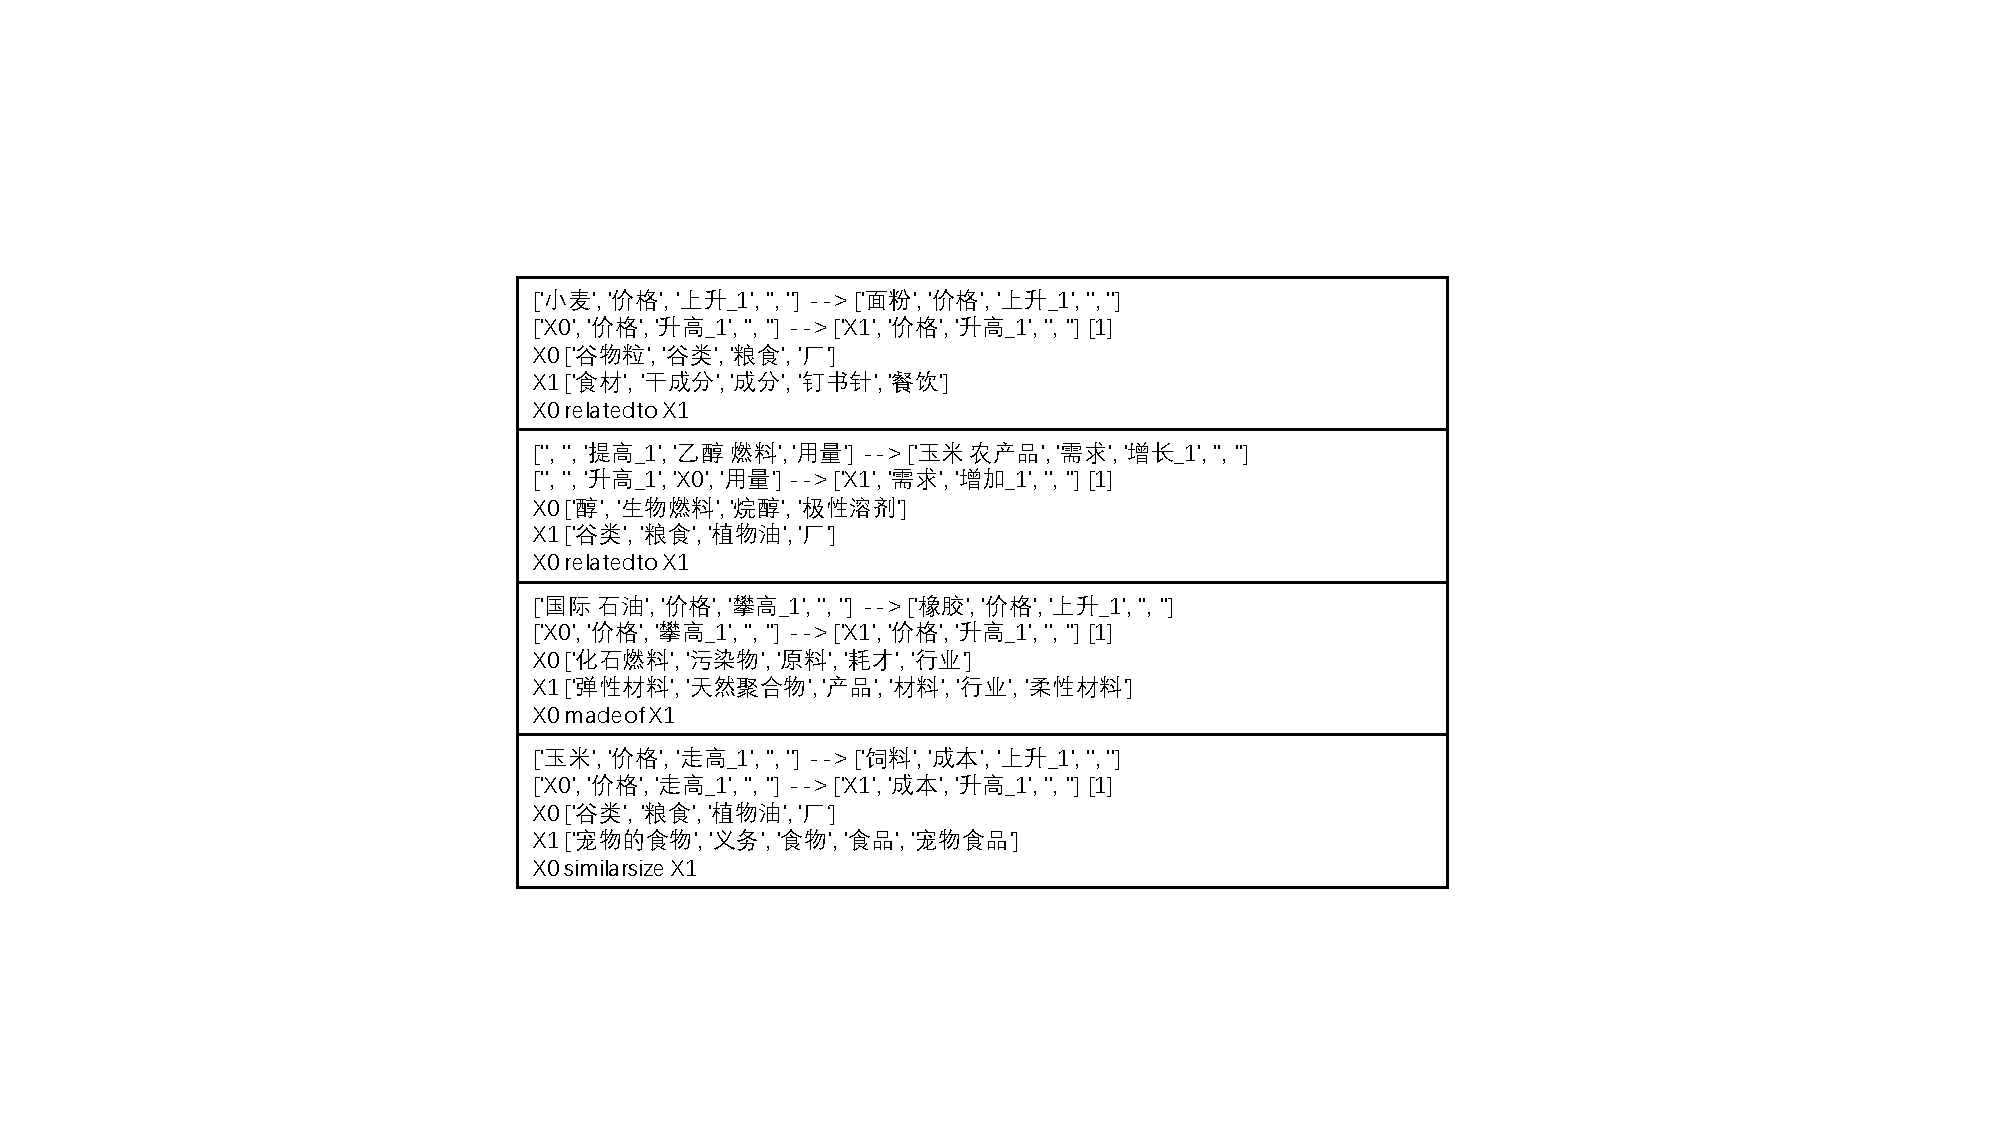
\includegraphics[width=0.95\columnwidth]{figures/reasonable_rule_case}
%	\end{center}
%	\caption{Examples of reasonable Rules.}
%	\label{fig:reasonable_rule_case}
%	\end{figure}
\begin{figure}[htbp]
	\centering
	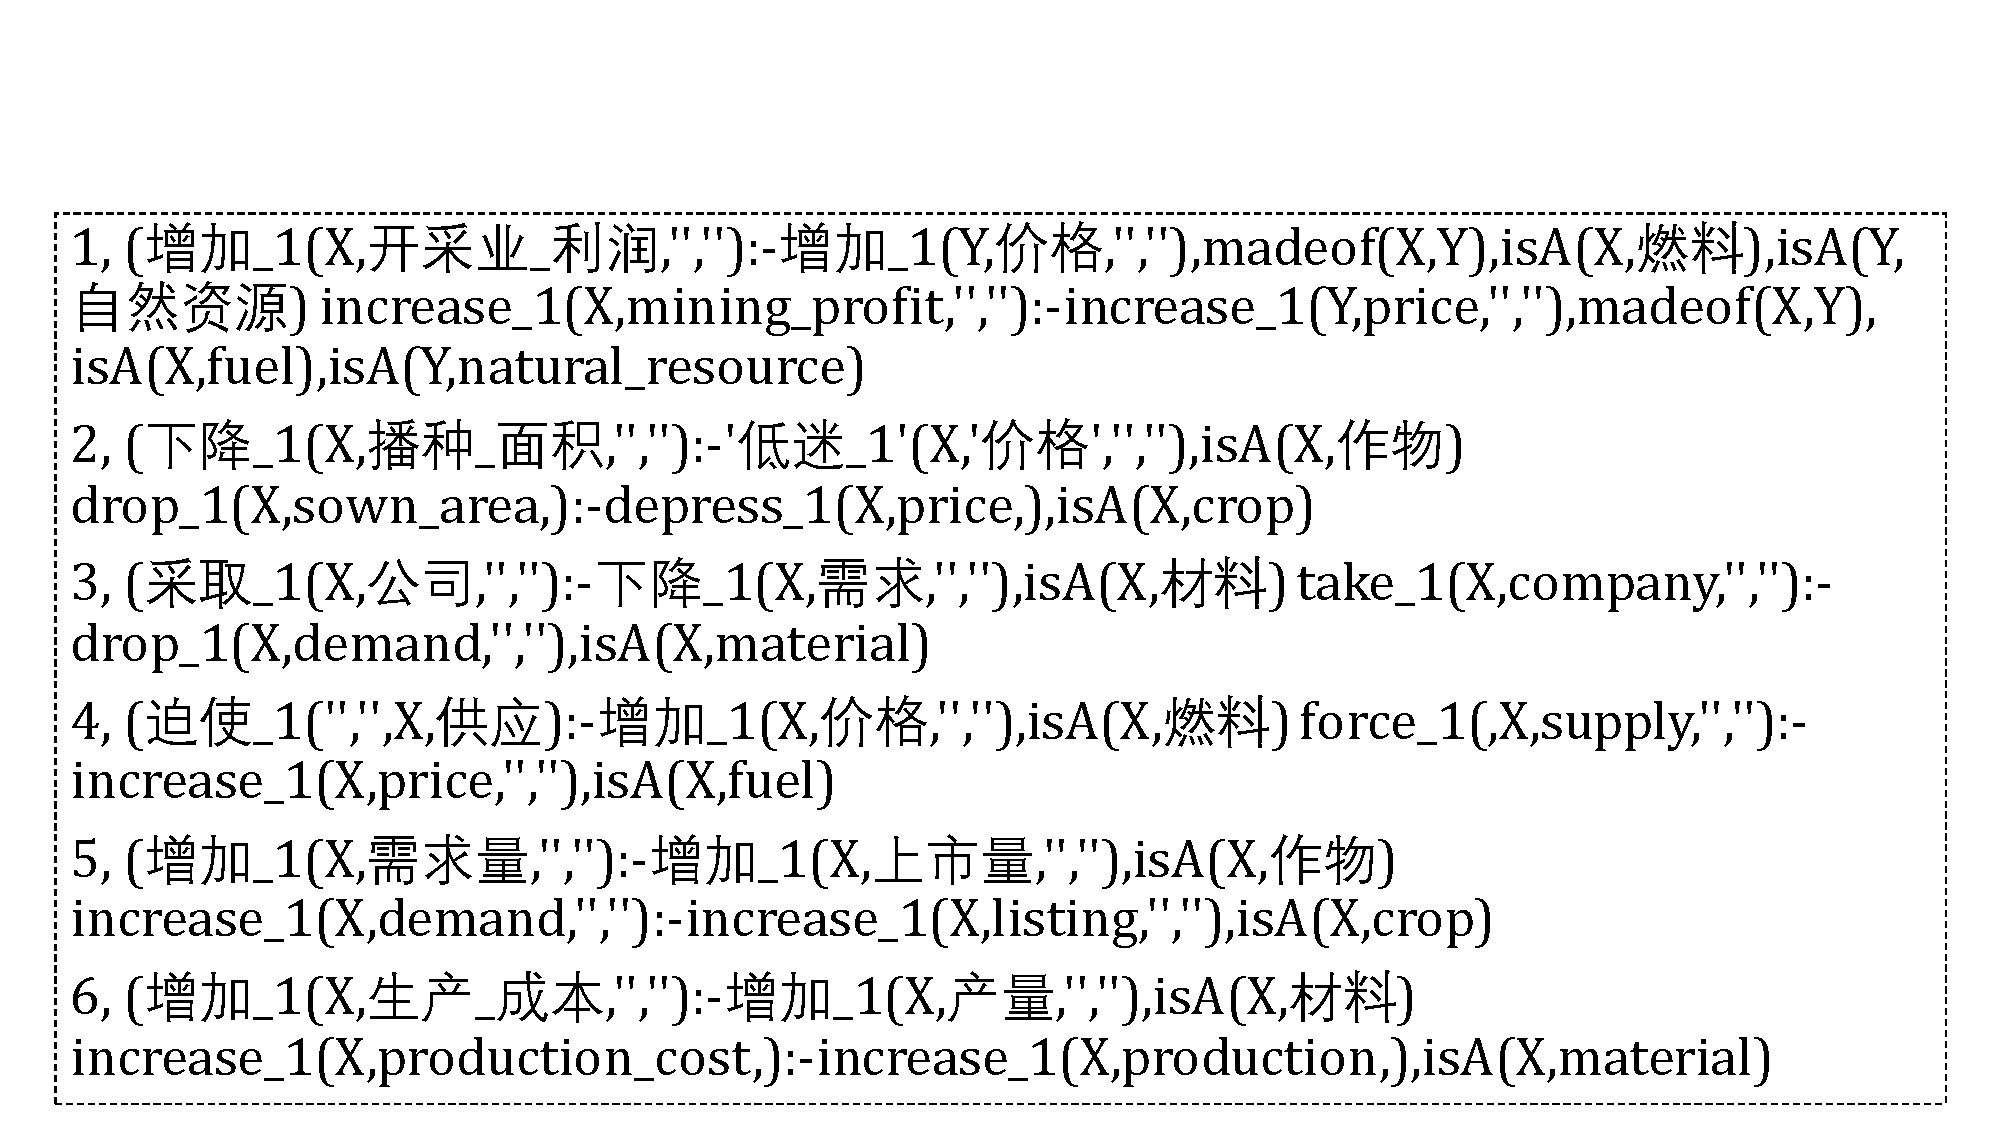
\includegraphics[width=0.95\columnwidth]{figures/rules_case}
	\caption{Examples of Typical Rules}
	\label{fig:rules_case}
\end{figure}
\paragraph{Event Graph}
With these rules, we deduce many rule instances with Prolog and pick out a tiny subgraph about rise and fall events, in Figure\ref{fig:rule_instantiation_graph}, to show the power of the rules. 
	
\begin{figure}[htbp]
\begin{center}
	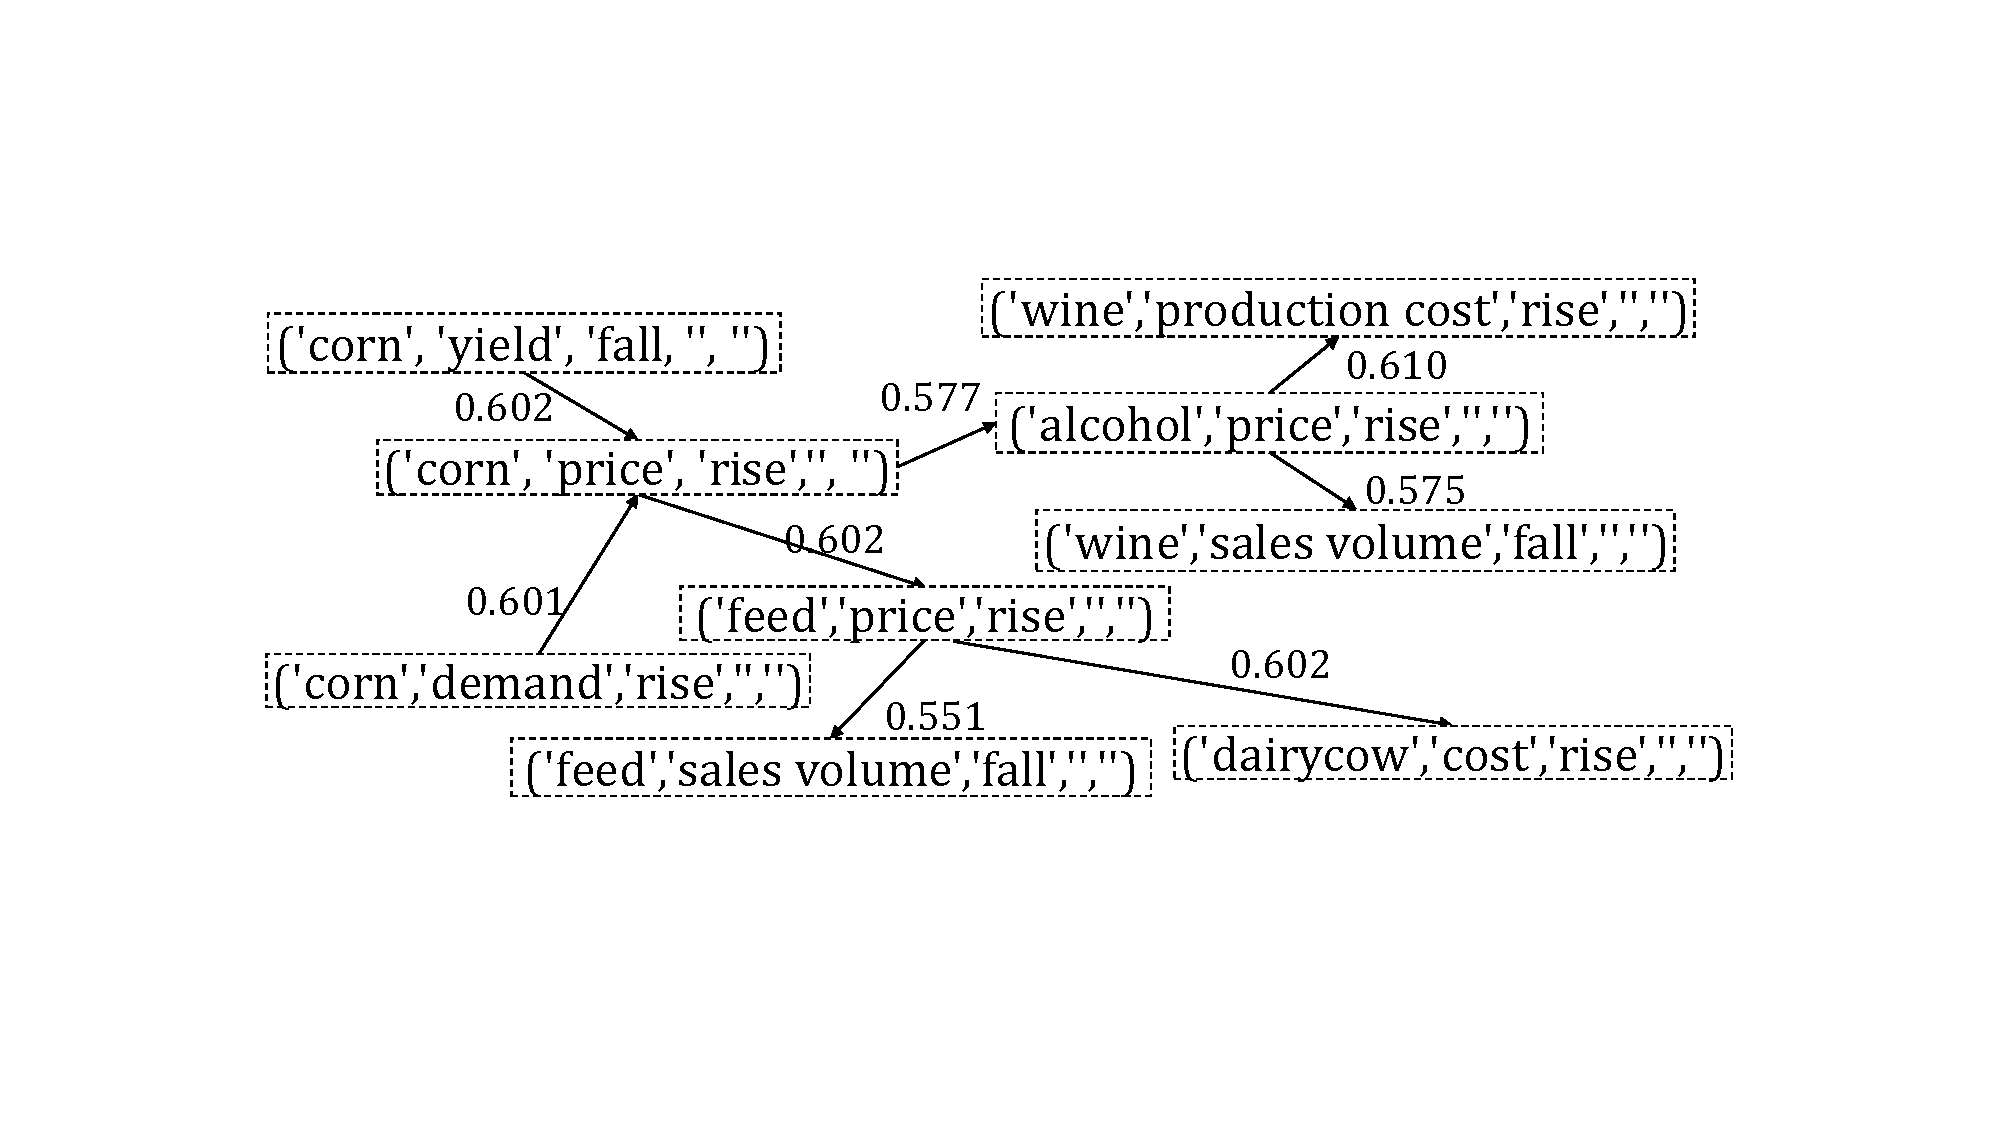
\includegraphics[width=0.9\columnwidth]{figures/instantiation_graph}
\end{center}
\caption{Rule Deduction. As space is limited, we only show the English version and omit the rules used in the reasoning process.}
\label{fig:rule_instantiation_graph}
\end{figure}

\subsection{Comparison with existing Knowledge Bases}
We compare our rules with causal part of other knowledge bases in various aspects in Table \ref{tab:comparison_rule_with_kbs}. We can see our causal knowledge representation is more expressive and informative, and the automatic knowledge acquisition is very convenient.
\begin{table*}[htbp]
\centering
%\begin{tabularx}{\columnwidth}{|c|c|c|c|}\hline
	\begin{tabular}{|c|c|c|c|c|c|c|c|}\hline
	\textbf{Name}&\textbf{Number}&\textbf{Domain}&\textbf{Unit}&\textbf{Data Structure}&\textbf{Information}&\textbf{Source}&\textbf{Precision}\\ \hline
	CausalNet&\textbf{62,675,002}&\textbf{Open}&word&(-)&rich&\textbf{automatic}&-\\
	\multicolumn{8}{|c|}{(`drink',`accident',36)}\\\hline
	ConceptNet &89,416&\textbf{Open}&short text&unstructured&rich&crowdsourcing&\textbf{100\%}\\
	\multicolumn{8}{|c|}{(`smoking',`/r/Causes',`cancer')}\\\hline
	FrameNet&59&\textbf{Open}&frame&\textbf{structured}&richer&crowdsourcing&\textbf{100\%}\\
	\multicolumn{8}{|c|}{Killing(Killer,Place,Means,Victim,Instrument),CausativeOf,Death(Protagonist,Place,Manner,Time)}\\\hline
	ATOMIC&568,312&\textbf{Open}&\textbf{logic event}&semi-structured&much richer&crowdsourcing&86.2\%\\
	\multicolumn{8}{|c|}{If ``PersonX pays PersonY a compliment", Then ``PersonY will smile"}\\\hline
	Ours&50,000&Finance&\textbf{logic event}&\textbf{structured}&\textbf{richest}&\textbf{automatic}&32.5\%\\ 
%			Deductive Rule Instance&\TD{??}\\ 
%	\multicolumn{8}{|c|}{See above rule example in Figure\ref{fig:rules_case}}\\\hline
\multicolumn{8}{|c|}{(Z,`price',`rise',`',`'):-(`',X,`suffer',Y,`attack'),isA(X,`country'),isA(Y,`disaster'),isA(Z,`metal'),atLocation(Z,X) conf:0.842}\\\hline	
	\end{tabular}
%\end{tabularx}  \cite{sap2018atomic}
\caption{Comparison with existing knowledge bases}
\label{tab:comparison_rule_with_kbs}
\end{table*}



%\begin{table}[htbp]
%	\caption{Rule Instance \& Rule}
%	\begin{center}
%	\begin{tabular}{|r|l|}\hline
%		\multicolumn{1}{|c|}{Name}                  & \multicolumn{1}{c|}{Number} \\\hline
%		\multicolumn{1}{|c|}{Rule Instances}        & \multicolumn{1}{c|}{7835403} \\ \hline
%		\multicolumn{1}{|c|}{Rules}                 & \multicolumn{1}{c|}{69036}  \\ \hline
%		\multicolumn{1}{|c|}{more than on relation} & \multicolumn{1}{c|}{2499(3.6\%)}\\
%		\multicolumn{1}{|c|}{only one relation}     & \multicolumn{1}{c|}{66539(96.4\%)} \\
%		\hline
%		==                                          & 56449(84.8\%)                      \\
%		madeof                                      & 5659(8.5\%)                        \\
%		atlocation                                  & 1835(2.76\%)                       \\
%		partof                                      & 1061(1.59\%)                       \\
%		usedfor                                     & 954(1.43\%)                        \\
%		hasa                                        & 511(0.768\%)                       \\
%		derivedfrom                                 & 38(0.0571\%)                       \\
%		hasproperty                                 & 20(0.0301\%)                       \\
%		createdby                                   & 12(0.018\%)                        \\ \hline
%	\end{tabular}
%	\label{tab:rule_statistics}
%\end{center}
%\end{table}
	%Rule Instances & 1817014(4337755)\\
	%Candidate Rules & 86218(201359)\\
	%Rule & 18348(42246)\\

\subsection{Ablation Study}
In this section, we explore the contributions of the various components of our rule learning framework.
\paragraph{Causal patterns statistic} The matched sentences distribution over 3 groups of patterns is shown in Table \ref{tab:pattern_statistics}. All patterns in one group have different causal cue words literally but the same meaning. It shows the third pattern group is more rigorous than the first two groups but has lower usage. Probably because more logical thinking is needed when editing news using more rigorous patterns.

%		\begin{table}[htbp]
%		\caption{Causal patterns. A is a cause tokens span, and B is an effect tokens span. Word '因为' represents a group works like '由于,'是因为','因为','缘于','归因于','原因是','起因','鉴于', and word '所以' represents a group of words like '所以','因而','因此','故此','故而','因故','导致','招致','以致','引致','诱致','致使','造成','使得','从而','从而使','于是','为此'}
%		\begin{center}
%			\begin{tabular}{|c|c|} \hline
%				\textbf{Pattern}& \textbf{Priority}\\ \hline
%				因为 A, 所以B&1\\ \hline
%				A,所以 B&2\\ \hline
%				因为 A,B&3\\ \hline
%			\end{tabular}
%			\label{tab:causal_pattern}
%		\end{center}
%	\end{table}	
	
\begin{table}[htbp]
	\centering
	\begin{tabular}{|c|c|c|c|} \hline
		\textbf{Pattern template}& \textbf{Priority}&\textbf{Number}& \textbf{Rate}\\	\hline 
		因为 A,B&1&2000242&48.32\% \\ \hline 
		A,所以 B&2&1530311&36.96\% \\ \hline 
		因为 A, 所以B&3&576851&14.72\% \\	\hline
	\end{tabular}
	\caption{Number of sentences extracted by causal patterns. A is a cause span and B is an effect span. Word `因为' represents a group works like 由于,是因为,因为,缘于,归因于,原因是,鉴于, and word `所以' represents a group of words like 所以,因而,因此,故而,因故,导致,招致,以致,引致,诱致,致使,造成,使得,从而使,于是,为此}
	\label{tab:pattern_statistics}
\end{table}	
\paragraph{External Knowledge Bases}
The following is some statistics of external knowledge bases used in the rule learning framework. The size of the lexicon is 12,624, obtained from `Industrial classification for national economic activities'\footnote{\url{ http://www.stats.gov.cn/Tjsj/tjbz/hyflbz/}}, which determines which event role in the rule instance can be generalized. 
To our knowledge, most existing Chinese taxonomic knowledge bases, such as CN-Probase\cite{Xu2017}, zhishi.me\cite{Niu2011}, are constructed from online-encyclopedia, which suffer that the concepts inside are far less than Probase and they have no probabilistic character. So we translate Probase to get 11,292,493 Chinese `IsA' pairs.
To our knowledge, there exists no large-scale Chinese commonsense knowledge base, so we translate the English part of ConceptNet and merge the Chinese part to get 2,085,681 Chinese triples.
We randomly sample 500 items from translated Probase and ConceptNet, respectively, and the accuracies after the human evaluation are \textbf{87.8\%}(close to the accuracy of original Probase 92.6\%) and \textbf{91.6\%}.

%\begin{table}[htbp]
%	\centering
%	\begin{tabular}{|c|c|}\hline
%		\textbf{Name}&\textbf{Number}\\ \hline
%		Lexicon&12624\\ \hline
%		Translated Probase &11,292,493(87.8\%)\\ \hline
%		Translated ConceptNet&2,085,681(91.6\%)\\ \hline
%	\end{tabular}
%	\caption{External Knowledge Bases}
%	\label{tab:knowledge_base_statistics}
%\end{table}

%After translation, the number of Chinese IsA pairs is 11,292,493. The number of Chinese commonsense triples is 2,085,681. We both randomly sample 500 items from them, and the accuracy after human evaluation are 0.878 and 0.916 respectively.
%The accuracy of original Probase is 0.926. 
%The number of total Chinese IsA pairs are 11,292,493 which contain concept-instance pairs and concept-subconcept pairs, the. The number of Chinese concepts is 81082 concluding concepts and subconcepts. The number of instances is 158693. The number of Chinese commonsense pairs is 7316977.
%\subsection{External Factual Knowledge Bases}

%From above rule instance extraction submodule, we scan get a rule instances repository. With such huge specific rule instances, we hope to further discover the powerful knowledge hidden in these rule instances. 

%so we generalize such a large amount of rule instances with a more general form. As discussed in Section \ref{sec:intro}, we need to build such a knowledge base. Taxonomy and common sense are two major kinds of knowledge in such knowledge base.
%In our framework, we need to rely on the external Chinese knowledge bases, Chinese Probase and Chinese Conceptnet, to generalize rule instances and add constraints. Most existing Chinese taxonomy knowledge is constructed from online-encyclopedia, such as CN-Probase\cite{Xu2017}. They usually focus more on named entity such as famous movie stars, singer stars, while we care more about the concrete things existed in life such as corn, steel, alcohol and so on.  In addition, they have no probabilistic character. Translation is an effective and efficient approach, we choose to translate Probase, which is a probabilistic taxonomic knowledge base.
%To our knowledge, there exists no large-scale Chinese commonsense knowledge base, so we translate the English part of ConceptNet5 into Chinese and combine the Chinese part.

%	 which is special for this, But it is only for English. We have investigated the CN-Probase\cite{xu2017cn}, but It even can't find the concept of common entities like '中国/China', '橡胶/rubber' and it also limits the usage frequency. So we collect the items from Probase, the items with 'IsA' relation in ConceptNet5\cite{speer2013conceptnet}, Webbrain\cite{chen2016webbrain}. Then, we fuse them together, Then, translate them into Chinese with google translator. to reduce the translate error, we put more context into the translator as more as possible, for example we put 'fruit such as apple, banana', Then we can get the translated result of IsA(apple,fruit), IsA(banana, fruit) together, which can make word sense of 'apple' to be translated near the fruit not company.  
%	\subsubsection{Chinese Commonsense knowledge base.}
%	, consisting of 47, 3, 25 relations respectively. Some of them are duplicative and some are useless for us. So we select specific number useful relations and we also design some patterns to extract some relations from Chinese wiki. 
%	relattions between arguments are used in rule specialization submodule to make rules reasonable. There exist many commonsense knowledge bases such as ConceptNet5, WebBrain, WebChild.  The numbers of the relations in these knowledge bases are limited. And some relations are equivalent among different knowledge bases, such as '/r/RelateTo' in ConceptNet is equivalent to 'relateto' in WebBrain. So we normalize all the relations names literally.
% Meanwhile, many pairs of arguments have more than one relations which are  duplicated semantically. For example, (sweet corn, corn) has the relations 'relatedto' and 'partof', obviously, 'partof' consists of 'relatedto' semantically. So we hope to remove the semantic reduplication relations. which means we need find the semantic containment relations among these relations.
%Algorithm \ref{alg:alg1} shows the Relations Containment algorithm we proposed. It firstly counts each relation and its corresponding arguments pairs. Then, compare the every two correlated relations, and record their containment relation. Last, enumerate all relations in each pair of arguments, remove the relation which is not contained in other relations existed in this pair of arguments.
%When fusing these knowledge bases, we regard arguments from different knowledge bases which have the same literal name as the same arguments.
%	from structured information to knowledge which is close to intelligence
%The goal of rule acquisition is to learn first-order logic rule from huge number of rule instances with the support of external factual knowledge, shown in the Figure \ref{fig:overview}'s middle part.
%with the knowledge base, now, we can generalize the rule instances extracted from rule instances extraction submodule into candidate rules to represent more general knowledge. For example, we hopefully generalize from each cluster of rule instances to one candidate rule. For example, given two rule instances in one cluster, ('国际 石油', '价格', '攀高@攀高', '', '') $->$ ('橡胶', '价格', '上升@升高', '', '') and ('国际 柴油', '价格', '攀高@攀高', '', '') $->$ ('橡胶', '价格', '上升@升高', '', ''), the generalized candidate rule would be('X0', '价格', '攀高', '', '') $->$ ('X1', '价格', '升高', '', '') where 'X0' IsA' 化石燃料','原料' and  'X1' IsA '弹性材料' '天然聚合物'.


%\begin{table}[htbp]
%\centering
%		\begin{tabular}{|c|c|}\hline
%			\textbf{Name}&\textbf{Number}\\ \hline
%			Lexicon&12624\\ \hline
%			Concepts &18281\\	
%			IsA pairs &123547\\
%			Concept-subconcept pairs&18753\\
%			Concept-instance pairs&104794\\\hline
%			Commonsense Pairs&32593\\ 
%			Commonsense Relations&10\\ \hline
%		\end{tabular}
%		\caption{Knowledge Base}
%		\label{tab:knowledge_base_statistics}
%\end{table}
\paragraph{Open Event Extraction}
%	TextRunner/WOE,ReVerb,Ollie,ClausIE,SRL/AMR parsing/frame-semantic parsing,NestIE 
Since our event structure scheme is plain and straightforward, we choose the reliable Stanford CoreNLP tool to extract the rule instances.
%	rule instance  97/200(48.5\%)& 21/200(10.5\%) & 82/200(41.0\%) \\ \hline
The number of rule instances extracted after rule instance distilling submodule is 7,835,403. Since most of them are discarded in the learning process, the number of rule instances really used for rule induction is 78,098 with an accuracy of \textbf{48.5\%} (we also sample 200 rule instances and manually evaluate them).

%\textit{To sum up}, our framework is a pipeline, in which rule instance extraction achieve 48.5\%, ConceptNet5 translation achieve 91.6\% and Probase translation achieves 87.8\%, So teh rule finally can achieve 39.0\%(48.5\%*91.6\%*87.8\%) maximumly, which is close to the evaluation of the final rules. 

%\textbf{\textit{To sum up}}, 
%our framework is a pipeline, in which the accuracy of rule instance extraction is 48.5\%, the accuracy of ConceptNet5 translation is 91.6\%, and the accuracy of Probase translation is 87.8\%. 
\textbf{\textit{To sum up}}, our framework is a pipeline undergoing rule instance extraction(accuracy 48.5\%), constrain relations addition(accuracy of ConceptNet 91.6\%), and rule induction(accuracy of Probase 87.8\%).
Thus, the accuracy can only reach \textbf{39.0\%} (48.5\%*91.6\%*87.8\%) at the maximum, which is close to our evaluation(32.5\%) of the final rules.

%	\subsubsection{Rule Acquisition}
%	\begin{table}[]
%		\centering
%		\begin{tabular}{lll}
%			& rule number  & qualitity       \\
%			no Coneptnet / only one relation    & 66539/96.4\% & informative     \\
%			Conceptnet / more than one relation & 2499/3.6\%   & more infrmative
%		\end{tabular}
%		\caption{Relation Number}
%	\end{table}

%	\begin{table}[]
%		\caption{Event Connection}
%		\begin{center}
%		\begin{tabular}{lll}
%			==         & 60475 & 84.4\%  \\
%			madeof     & 6161  & 8.6\%   \\
%			atlocation & 2104  & 2.94\%  \\
%			partof     & 1152  & 1.61\%  \\
%			usedfor    & 1072  & 1.5\%   \\
%			others     & 674   & 0.941\%
%		\end{tabular}
%		\end{center}
%	\end{table}
\subsection{Application: Futures Price Prediction}
%\paragraph{Reasoning with Uncertainty}
\begin{figure}[htbp]
	\begin{center}
		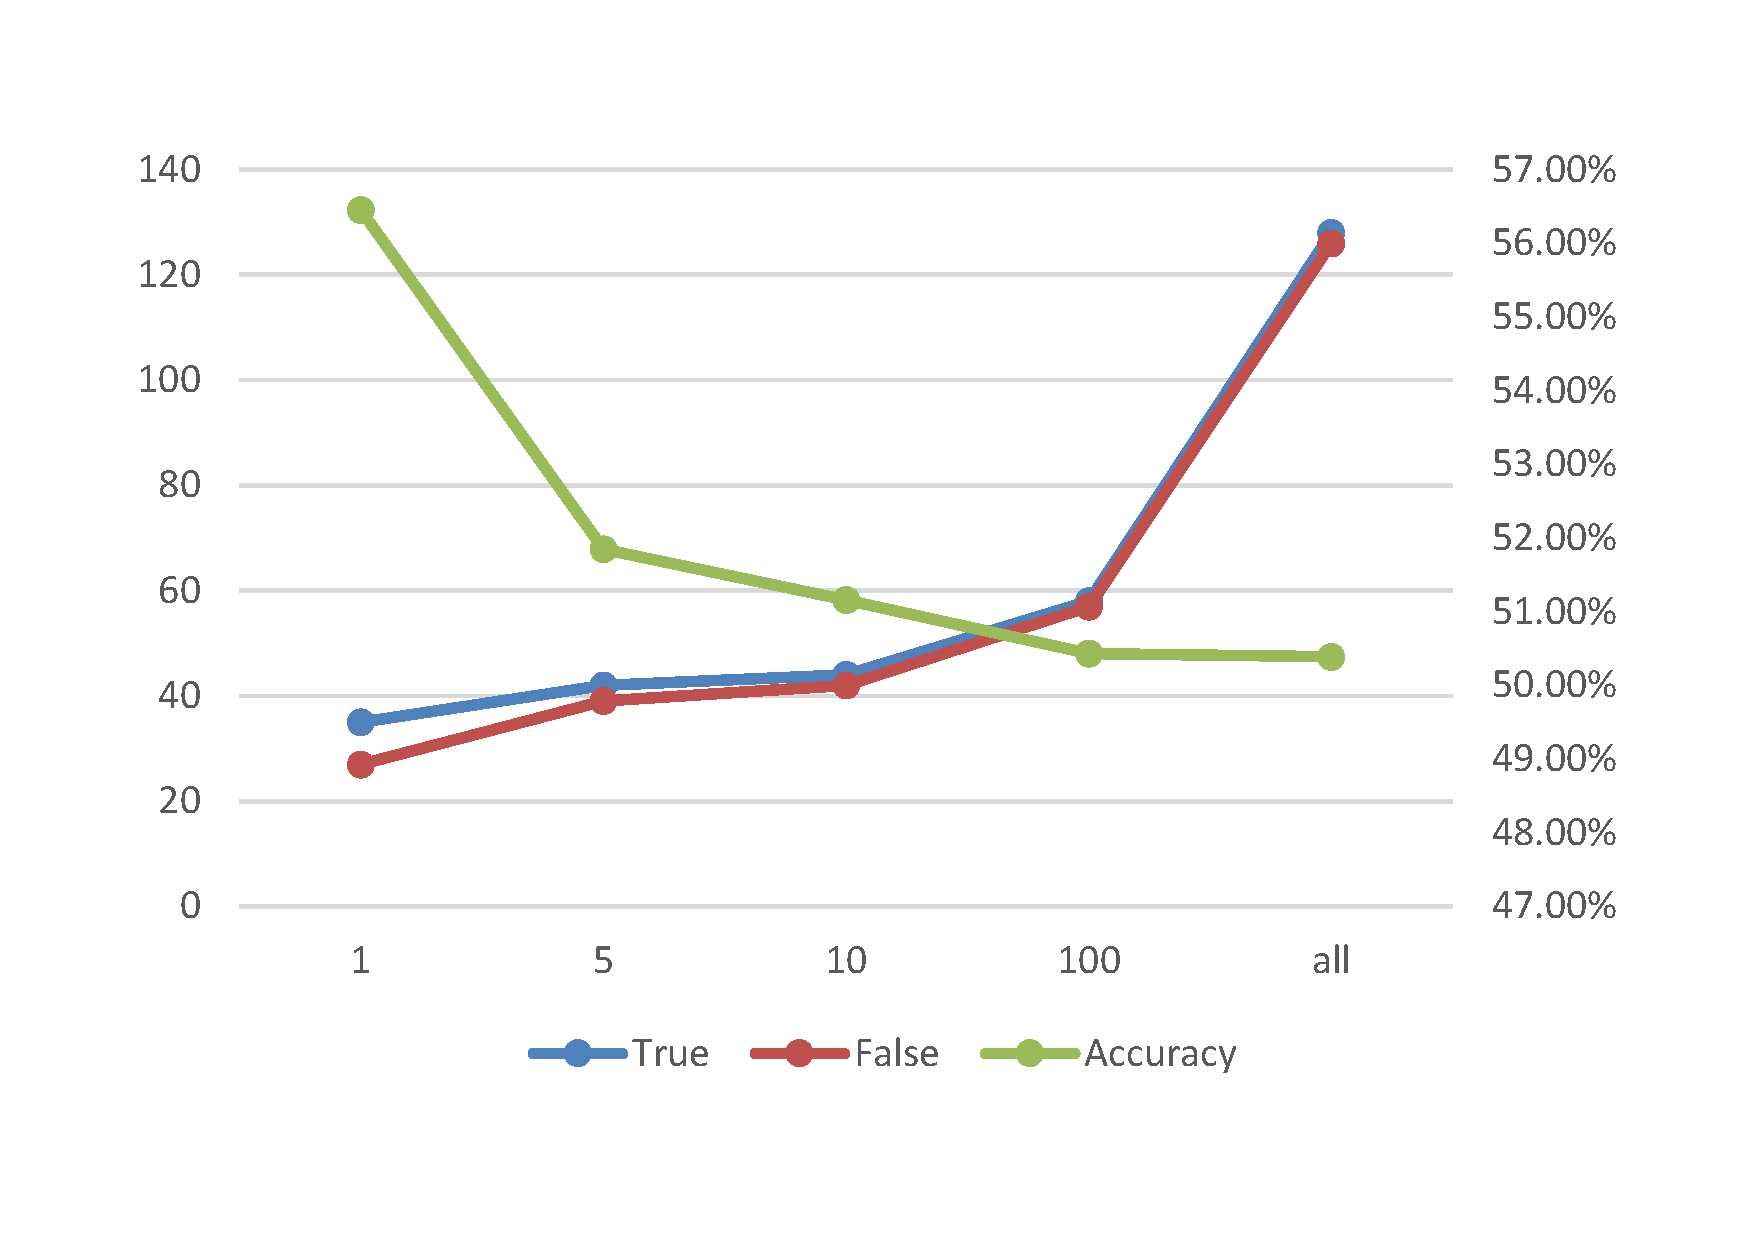
\includegraphics[width=0.9\columnwidth]{figures/rule_futures_prediction}
	\end{center}
	\caption{Futures Price Prediction.}
	\label{fig:futures_price_prediction}
\end{figure}
We choose futures price prediction because the futures are common and concrete things existed in ConceptNet and Probase, such as corn, oil, etc.
%\cite{Ding} is the state-of-the-art stock prediction model(EB\_CNN). We follow similar experimental settings. 
We follow similar experimental settings in \cite{Ding}.
From 2018/1/1 to 2018/11/2, we collect all the headlines and the price change of 15 futures as test data, which include \textbf{851} price change events (The price change of more than 1\% relative to the previous day is an event and we only focus on rise or fall events). 

Baseline models: EB\_CNN model \cite{Ding}, the state of the art model in stock price prediction, uses a deep convolutional neural network to model both short-term and long-term influences of events on stock price movements, and the accuracy of futures prediction is \textbf{54.2\%}. Other models in \cite{Ding}, such as EB\_NN, WB\_CNN, and WB\_NN can achieve \textbf{53.0\%}, \textbf{53.2\%}, and \textbf{53.5\%}, respectively. These accuracies of futures prediction are lower than the accuracies of stock prediction shown in the paper.
It may be because the factors affecting the futures price are far less than the stock price and the futures price is much more stable than the stock price, which makes useful training information about the futures less and further affects the accuracy of the models.

Our approach: For each actual future price change event , we get the news headlines for the previous month before this event. 
For each news headline, we extract the event, use Prolog to reason based on the rules and external knowledge bases, and get the top K inferred events sorted by the confidence.
We may have m*K inferred events for this event, m is the number of events occurred in this month. 
Here, we select the price change events(rise or fall) of the future in this actual future price change event from m*K events and calculate the weighted sum of their confidences(rise event weights 1 and fall event weights -1). If the sum value is positive, we predict this future price as a rise event, otherwise as a fall event. If get no related events changing the future's price, do not make prediction. We compare this prediction with the actual price change to evaluate the reasoning effect. 
Figure \ref{fig:futures_price_prediction} shows the average prediction result. It shows the more predicted events inferred from the Prolog(by increasing K) we use, the lower the prediction accuracy is(from \textbf{56.5\%} to \textbf{50.4\%}), and the more futures events we can predict(from \textbf{62} to \textbf{254}). 

\textbf{\textit{To sum up}}, our rule-based prediction approach can have a higher prediction accuracy (56.45\%) and better interpretation ability with a low recall rate, which is very practical in life.

%\begin{table}[htbp]
%	\caption{Baselines and Proposed Framework}
%	\begin{center}
%		\begin{tabular}{lll}\hline
%			& Acc & MCC \\\hline
%			WB-NN &  0.535 &     \\
%			WB-CNN&  0.532  &     \\
%			EB-NN &  0.530  &     \\
%			EB-CNN&  0.542   &     \\
%			Rule &     &    \\\hline
%		\end{tabular}
%		\label{tab:baselines_and_rule}
%	\end{center}
%\end{table}

\subsection{Downloading and Demo}
The translated Chinese Probase and ConceptNet and learned rules are available at URL.
We built a demo to demonstrate the reasoning process at URL. 
We also developed an application demo of futures prices change triggering that can monitor news from around the world in real time, find the news that may cause futures prices changes, and alert users. Visit URL.
\section{Related Work}
\paragraph{Clarification Question Generation} The concept of CQ can be naturally raised in a dialogue system where the speech recognition results tend to be erroneous so that we raise CQs for sanity check \citep{stoyanchev2014towards}, or the intents for a task is incomplete or ambiguous in a first short utterance and further CQs are needed to fill in the slots \citep{dhole2020resolving}. The concept is then extended to IR to clarify ambiguous queries \citep{aliannejadi2019asking}, and has been successfully put into practice \citep{zamani2020generating}. Other application areas including KBQA \citep{xu2019asking} and open-domain dialogue systems \citep{aliannejadi2020convai3}. CQGen can also be applied to help refine posts on websites like StackExchange \citep{Kumar_2020} and Amazon \citep{rao2019answer}. In this context, our work closely follows the research line of \citep{rao2018learning, rao2019answer, cao2019controlling}. \citet{rao2018learning} first adopted a retrieval-then-rank approach. They \citep{rao2019answer} then proposed a generation approach to train the model to maximize the utility of the hypothetical answer for the questions with GAN, to better promote specificity. \citet{cao2019controlling} propose to control the specificity by training on data with explicit indicator of specificity, but it requires additional specificity annotation. Towards the similar specificity goal, we adopted a different keyword-based approach. They also assume generating one question per context, which we claim is not sufficient to cover various possible information needs, and thus propose the task of the diverse CQGen.

\paragraph{Diverse Generation} The demand for diverse generation exists in many other fields~\cite{vijayakumar2018diverse, LiangZ18code, shen2019mixture}, and we've drawn inspirations from these literatures. For image captioning, we may use multiple descriptions for different focusing points of a scene. \textit{Diverse Beam Search} \citep{vijayakumar2018diverse} was proposed to broaden the searching space to catch such diversity by dividing groups in decoding and imposing repetition penalty between them. For machine translation, a context can be translated with different styles. \citet{shen2019mixture} thus proposed \textit{Mixture of Expert} models including hMup to reflect various styles with a discrete latent variable (\textit{expert}). And here for CQGen, diversity is required to cover various potentially missing aspects, so we come up with the idea to use keywords as a controlling variable like \textit{expert} to promote diversity.


\section{Conclusion}

In this paper, we incorporated the idea of Cookie Theft picture description task into the evaluation of the high-level cognitive abilities of LVLMs and designed a novel evaluation benchmark called CogBench.
% Images in CogBench are of high quality and require more cognitive reasonings to understand, which makes it different from existing image datasets.
The images in CogBench are of high quality and demand more complex cognitive reasoning for interpretation, setting it apart from existing image datasets.
% It consists of a image description task and a VQA task.
Experiments show that there is still a large gap between the cognitive abilities of LVLMs and human beings, indicating CogBench is a challenging benchmark.

% In the future


%%
%% The next two lines define the bibliography style to be used, and
%% the bibliography file.
\bibliographystyle{ACM-Reference-Format}
\bibliography{references}

%%
%% If your work has an appendix, this is the place to put it.
% \appendix

% \section{Research Methods}

% \subsection{Part One}

\end{document}
\endinput
%%
%% End of file `sample-sigconf.tex'.
